\section{Scenario}
\subsection{Admin}
- The admin logs in to the website using their admin credentials. Once logged in, the admin is directed to the dashboard where they can see orders of website.The admin can then navigate to the different sections of the website, such as Products, Customer Care, Posts, Promotions, Customers, HRM, Statistic.\\
- In the orders section, the admin can view and manage orders that have been placed by customers. Admin can change the status of orders, update delivery details, and manage refunds or returns.\\
- In the products section, the admin can add, edit, or delete products from the website. Admin can also manage product categories, adjust pricing, and update product descriptions.\\
- In the customer care section, the admin can manage and solve support request from customer. Admin can reply the request, filter request.\\
- In the posts section, the admin can add new post, delete, edit post. In edit content of post, they can add tag for post, add image.\\
- In the promotions section, they can add new promotion, set status and expired date for promotions.\\
- In the customers section, the admin can view and manage customer's accounts. The admin can update status of customer's accounts.\\
- In the HRM, the admin can manage account of employee, the admin can add new employee with different roles. Besides, the admin can filter or search employee.\\
- In the Statistic section, the admin can view all statistic revenue and product purchased.\\
- The admin can also manage website settings such as shipping and payment options, website design, and website policies. Once the admin has made the necessary changes or updates, they can log out of the website.
\subsection{Customer}
- Visit the website: The customer navigates to the website and lands on the home page.\\
- Login: The customer logs in by email.\\
- View products: The customer browses through the available products and selects the desired products to purchase.\\
- Add to cart: The customer adds the selected products to the cart.\\
- Review cart: The customer reviews the cart, updates the quantities or removes products if needed.\\
- Checkout: The customer proceeds to checkout, enters the billing and shipping information.\\
- Payment: The customer selects the payment method and provides the necessary payment details.\\
- Place order: The customer reviews the order details and confirms the order.\\
- Order confirmation: The customer receives a confirmation message, and the order is placed.\\
- Order tracking: The customer can track the status of their order using the provided tracking information.
- Order delivery: The customer receives the order at the provided address.
\section{Demo}
\subsection{Login}
1. User navigates to the website's landing page at \href{https://coffee.skrt.cc}{here}. \\
2. Choose Login on the header \\
3. Choose Google account to login \\ 
\begin{figure}[H]
    \centering
    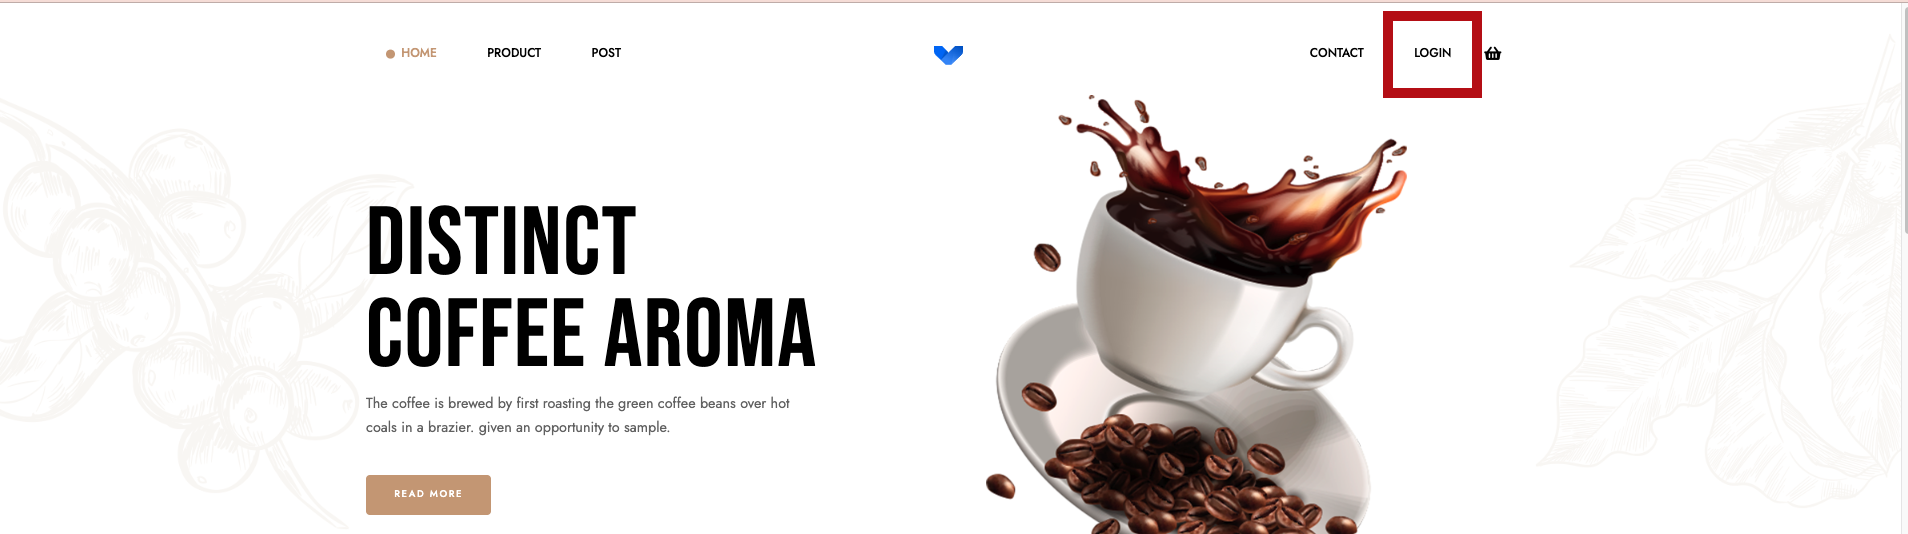
\includegraphics[width=0.7\textwidth]{Demo/Screenshot_2.png} 
    \label{fig:supportpage}
\end{figure}
\begin{figure}[H]
    \centering
    
\includegraphics[width=0.7\textwidth]{Demo/Screenshot_3.png}
    \label{fig:supportpage}
\end{figure}

\subsection{View statistics}
1. Login first \\
2. User navigates to the website's View statistic at \href{https://coffee.skrt.cc/admin/statistic/revenue}{here}. \\
3. User can choose date range to view\\
\begin{figure}[H]
    \centering
    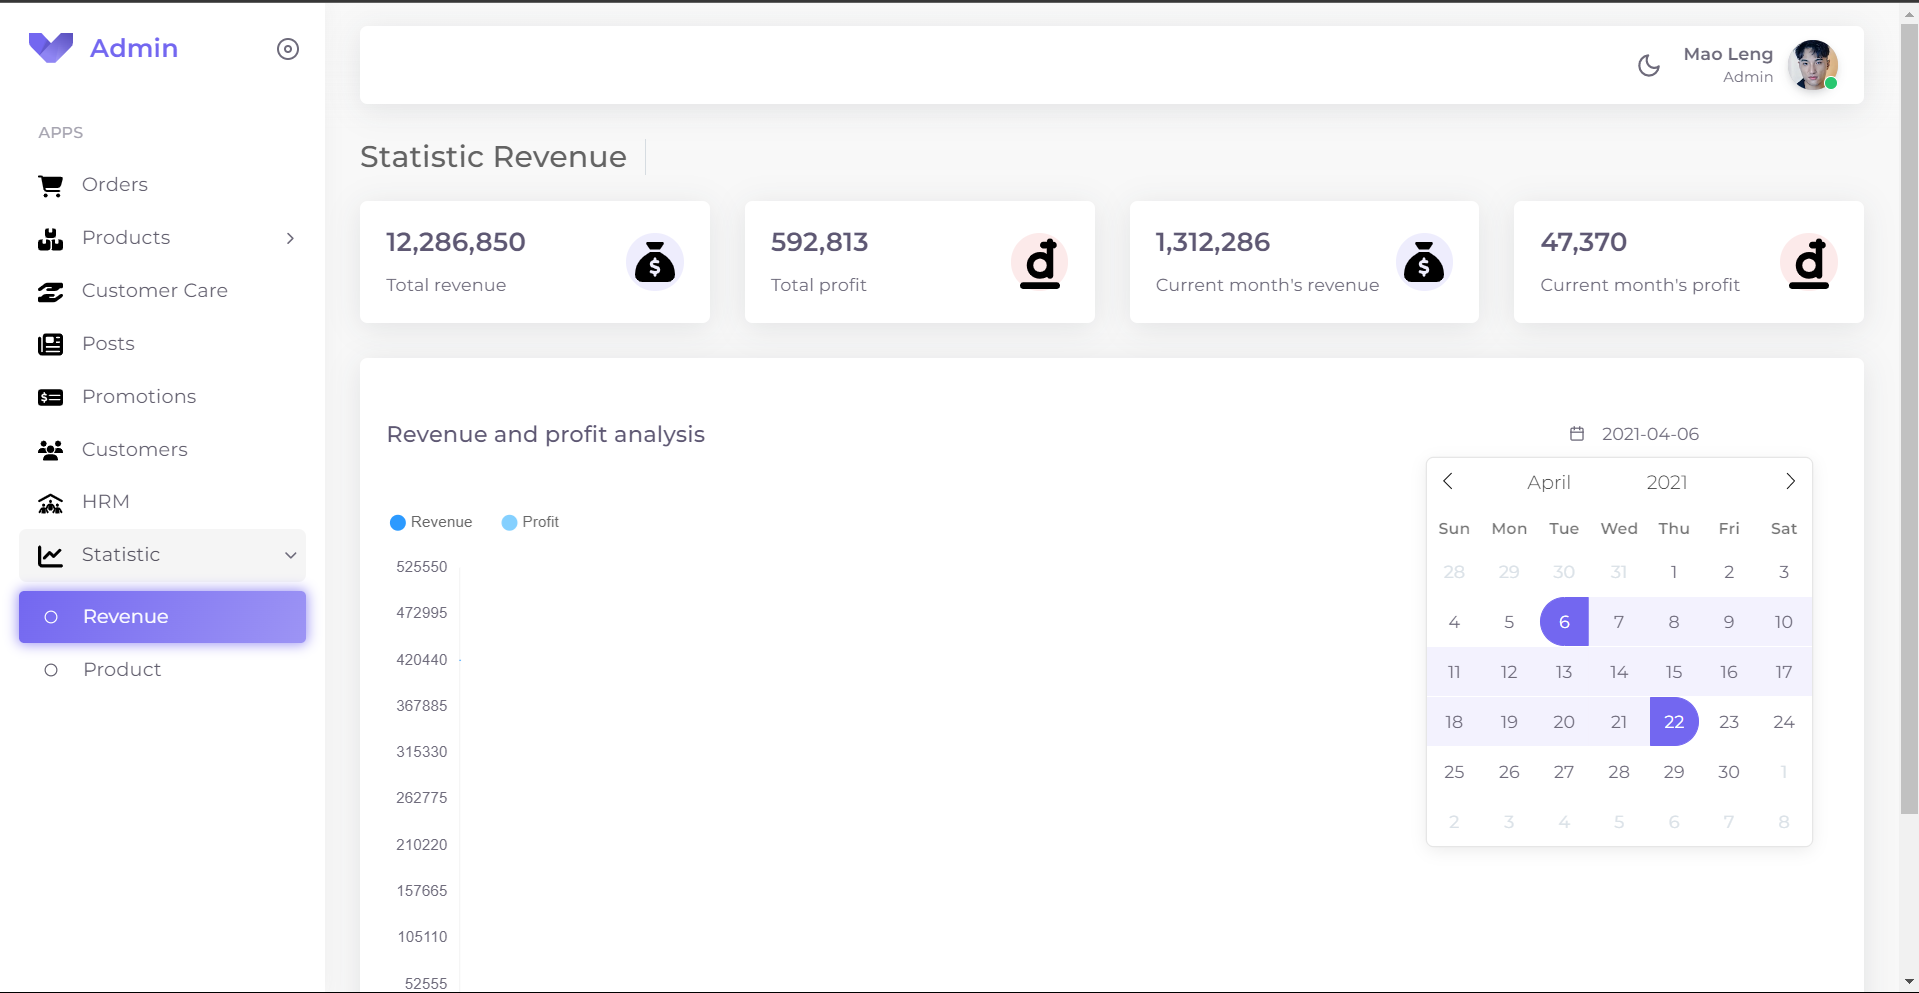
\includegraphics[width=0.7\textwidth]{Demo/Screenshot_4.png}
    \label{fig:supportpage}
\end{figure}
\begin{figure}[H]
    \centering
    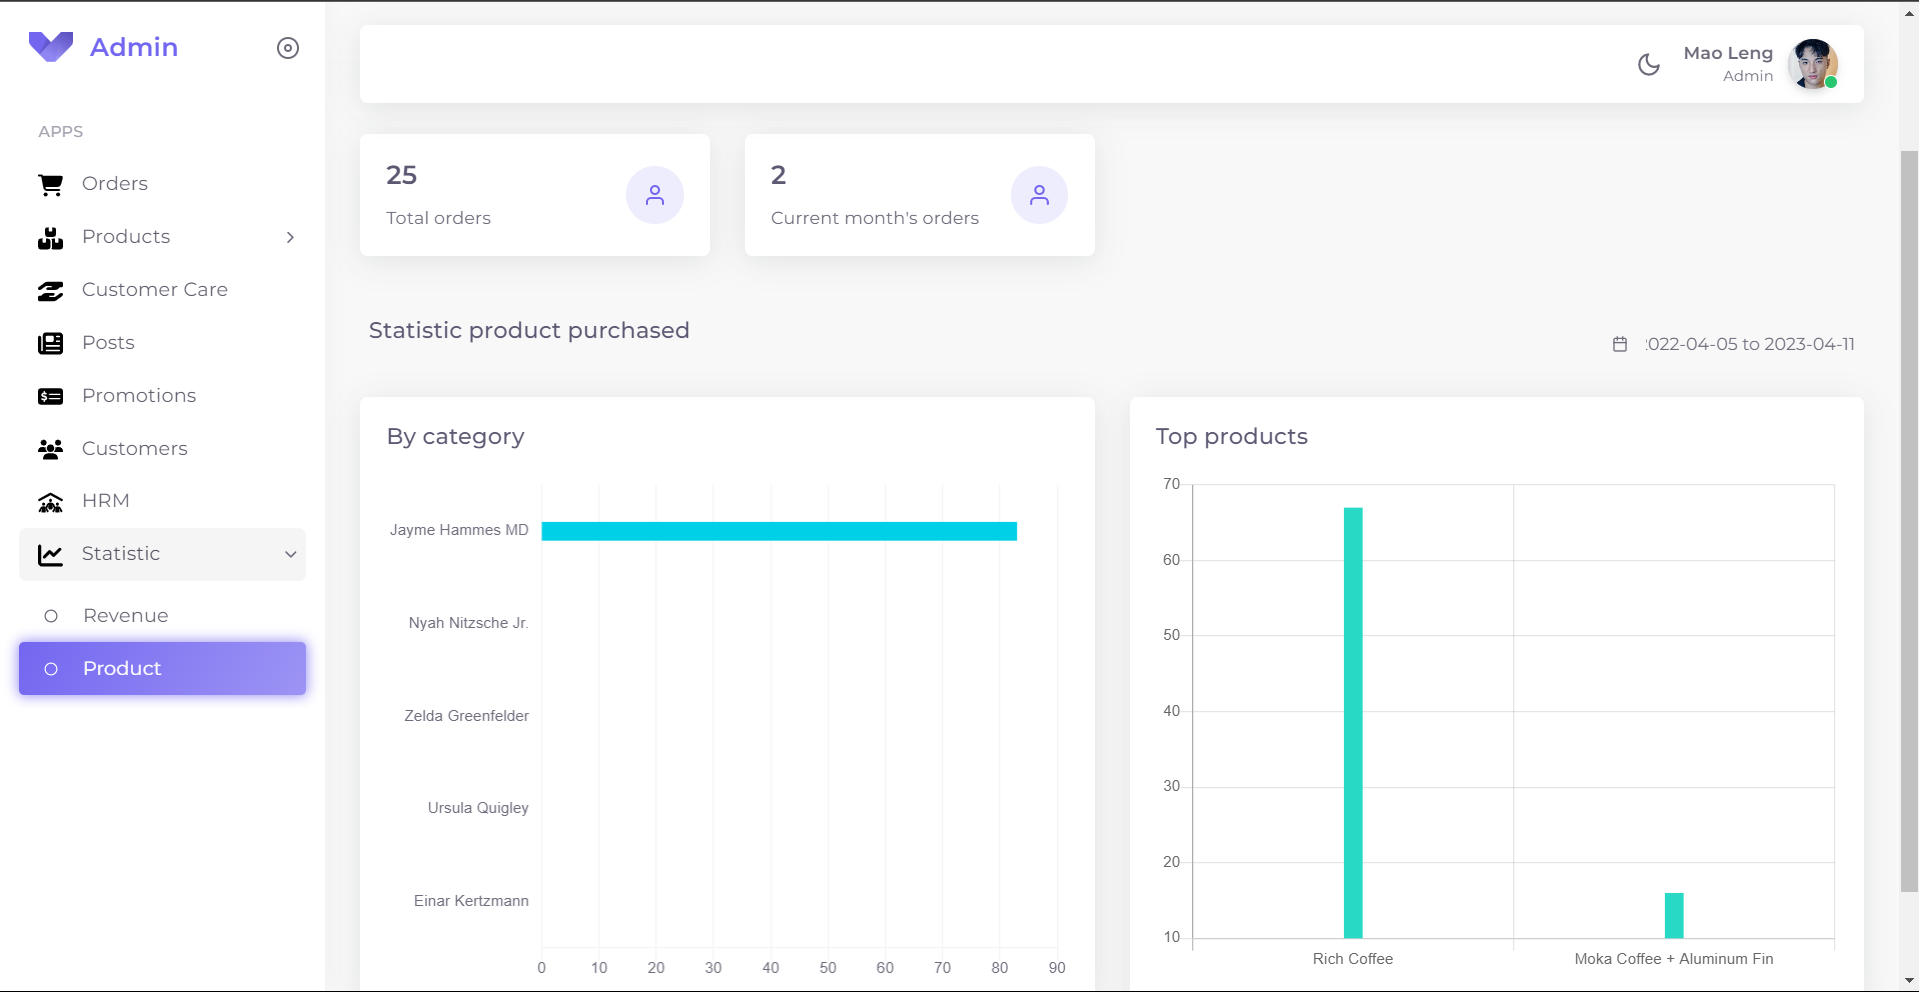
\includegraphics[width=0.7\textwidth]{Demo/Screenshot_5.png}
    \label{fig:supportpage}
\end{figure}


\subsection{Manage employee}
1. Login first \\
2. User navigates to the website's Manage employee at \href{https://coffee.skrt.cc/admin/hrm}{here}. \\
3. User can filter joined date by date range, filter by role or search by input\\
4. User can add new employee by click Add employee button, fill information, then click add\\
\begin{figure}[H]
    \centering
    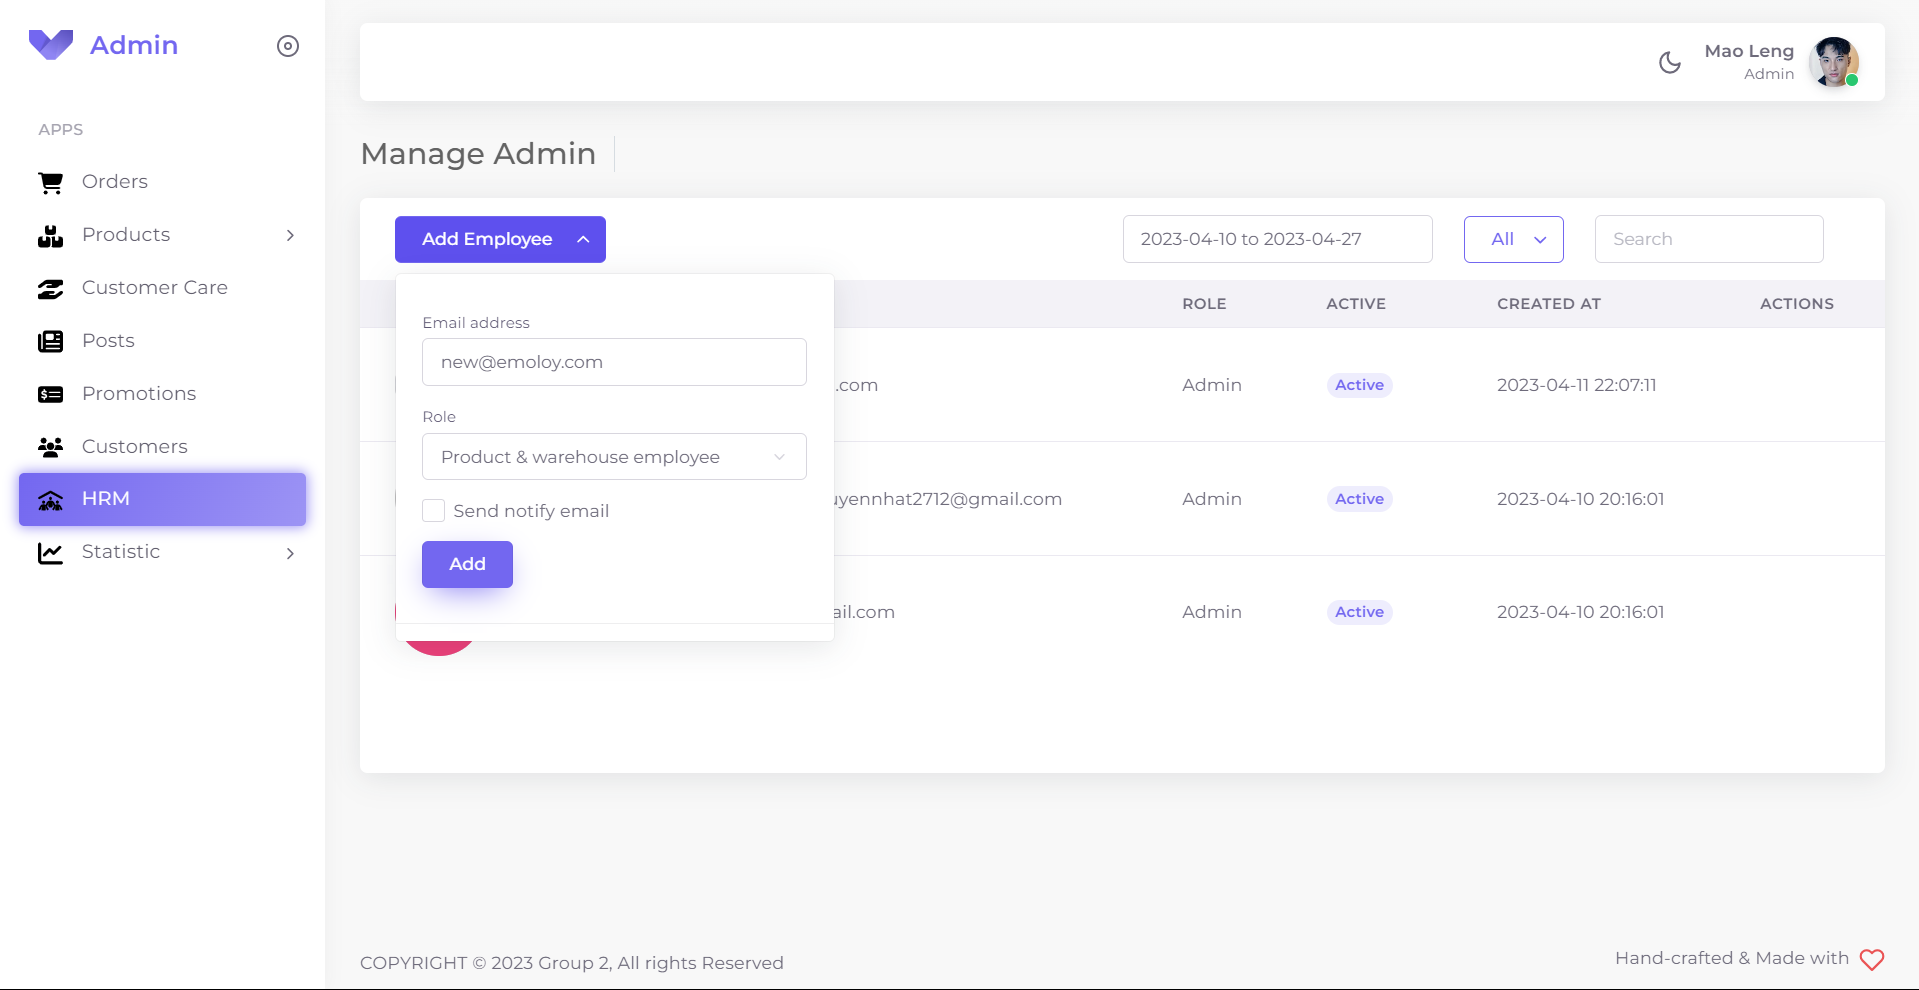
\includegraphics[width=0.7\textwidth]{Demo/Screenshot_7.png}
    \label{fig:supportpage}
\end{figure}

\begin{figure}[H]
    \centering
    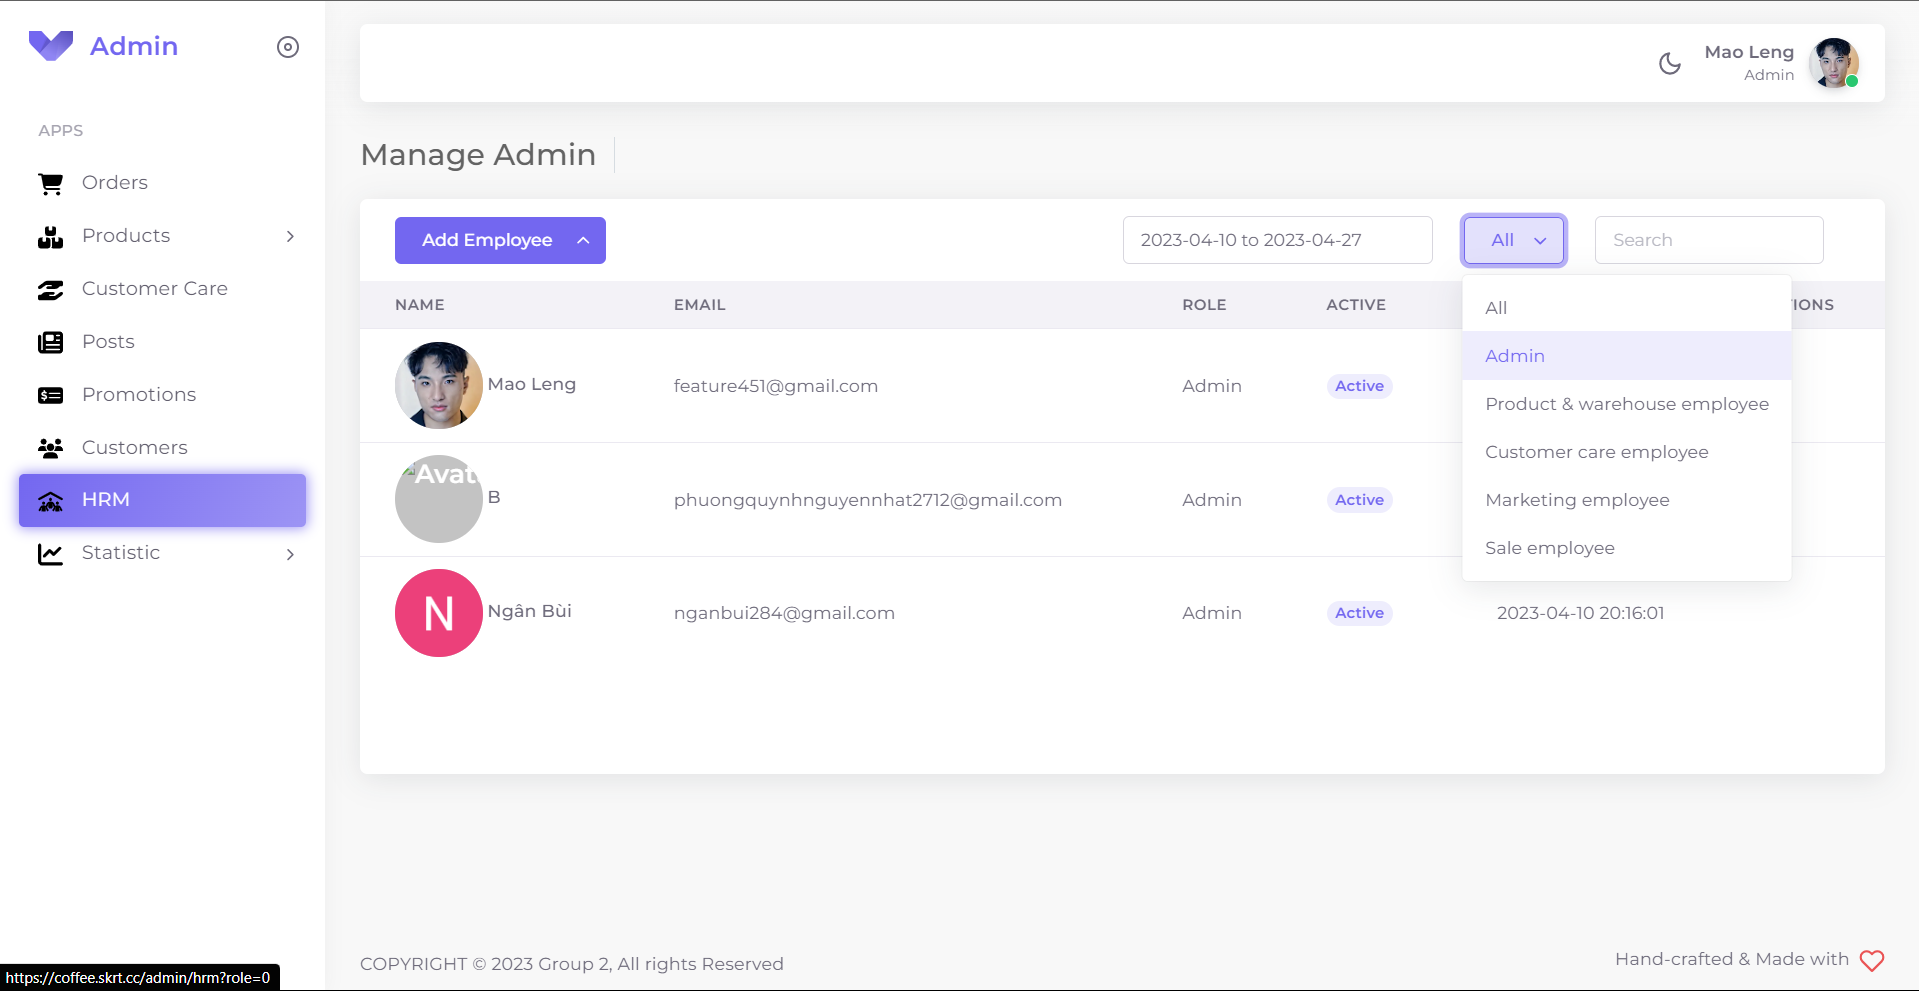
\includegraphics[width=0.7\textwidth]{Demo/Screenshot_6.png}
    \label{fig:supportpage}
\end{figure}
\subsection{Manage customer}
1. Login first \\
2. User navigates to the website's Manage customer at \href{https://coffee.skrt.cc/admin/customer}{here}. \\
3. User can search by input\\
4. User can see detail information by clicking view detail\\
\begin{figure}[H]
    \centering
    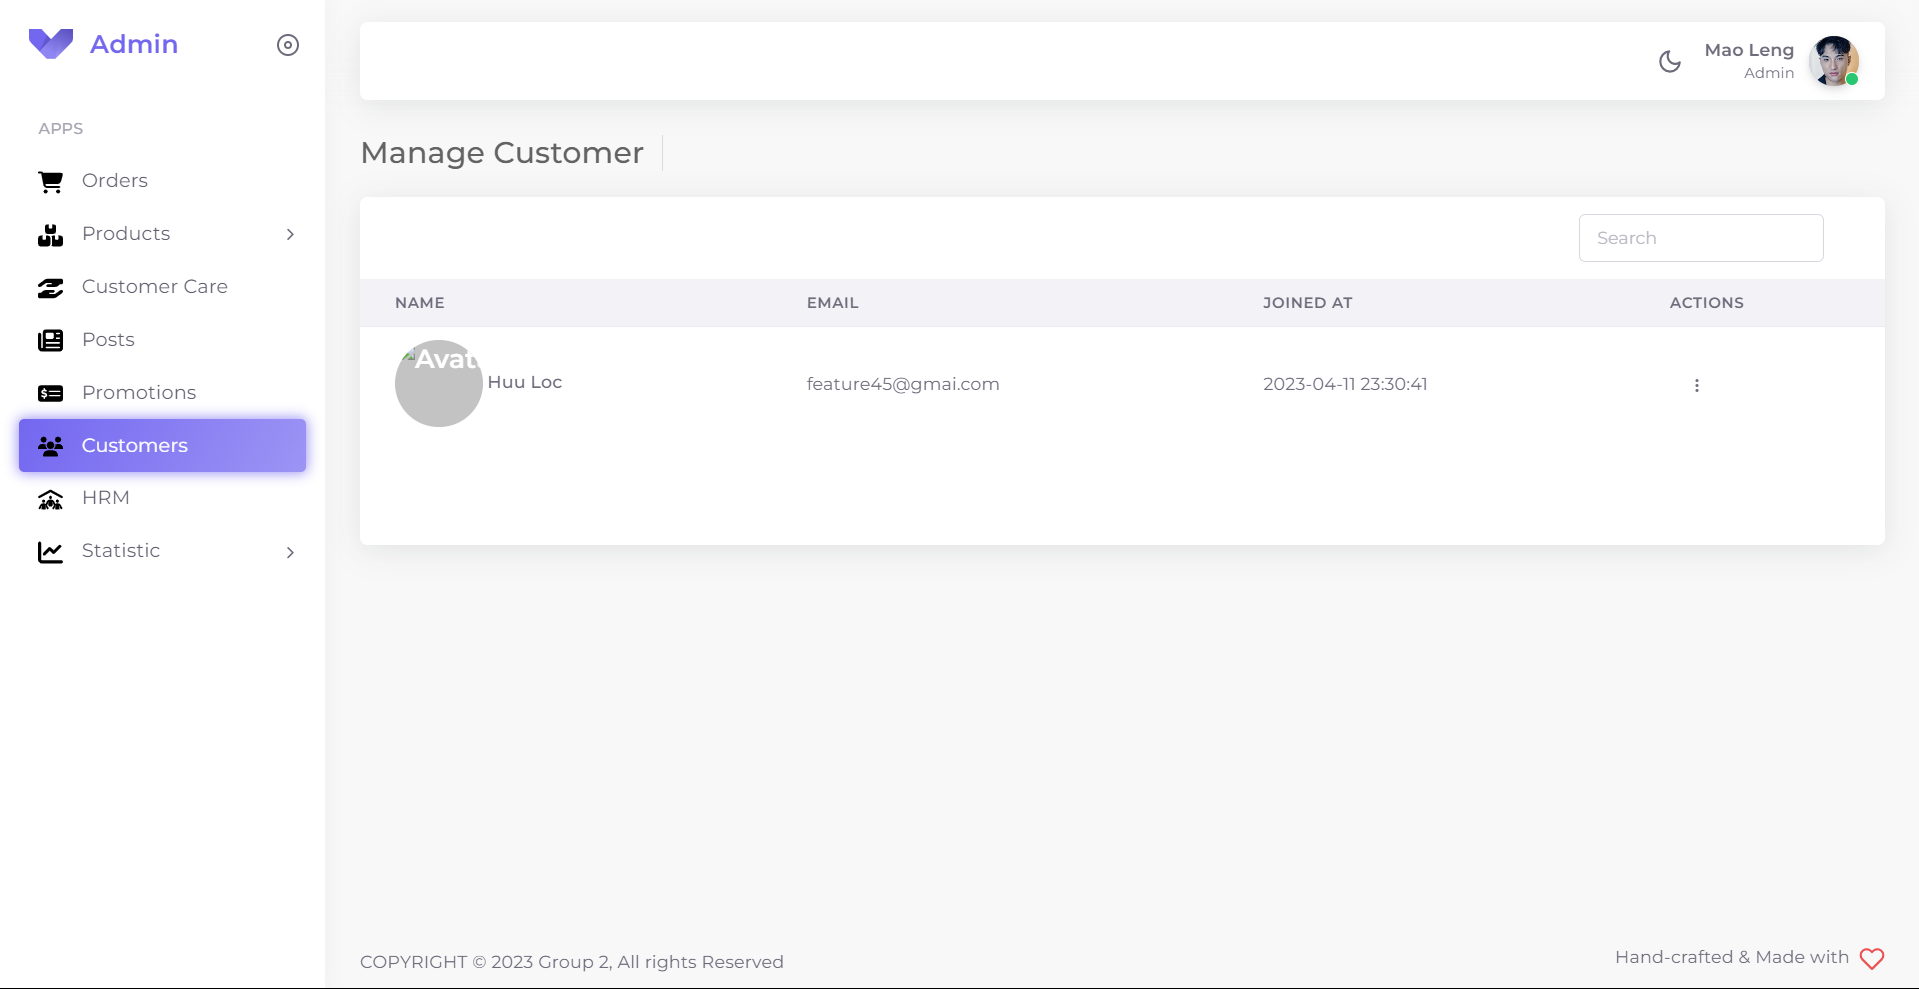
\includegraphics[width=0.7\textwidth]{Demo/Screenshot_8.png}
    \label{fig:supportpage}
\end{figure}
\begin{figure}[H]
    \centering
    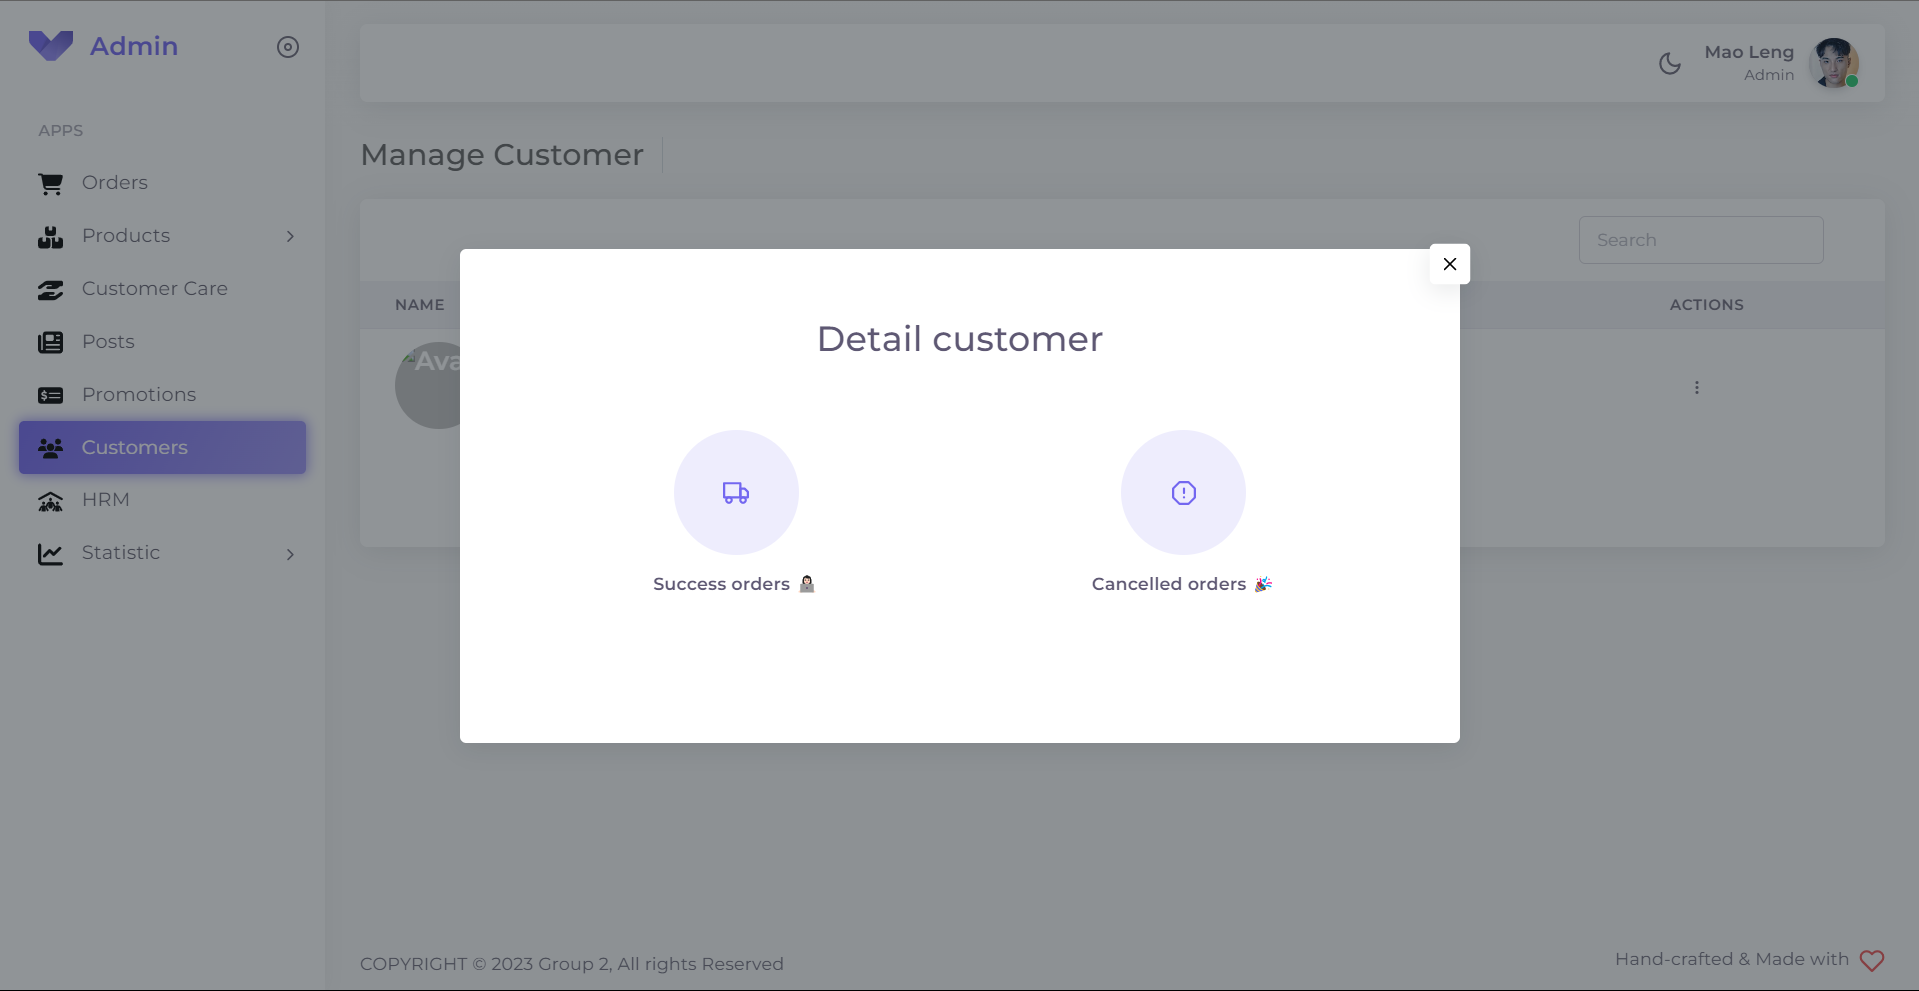
\includegraphics[width=0.7\textwidth]{Demo/Screenshot_9.png}
    \label{fig:supportpage}
\end{figure}

\subsection{Manage product and repository}
1. Login first \\
2. User navigates to the website's Manage product and repository at \href{https://coffee.skrt.cc/admin/warehouse}{here}. \\
3. User can search by input, filter by time range, filter by category\\
4. User can edit product's information by clicking edit on actions, fill the new data, then click save.\\
5. User can store product's information by clicking Add product button, fill the data, then click save.\\
6. User can delete product by clicking Delete on actions.\\
7. User can import product by clicking Import Product button, then choose supplier, fill input information with its amount and price.\\
8. User can Manage the supplier by CRUD, navigate to  \href{https://coffee.skrt.cc/admin/supplier}{here}.\\
\begin{figure}[H]
    \centering
    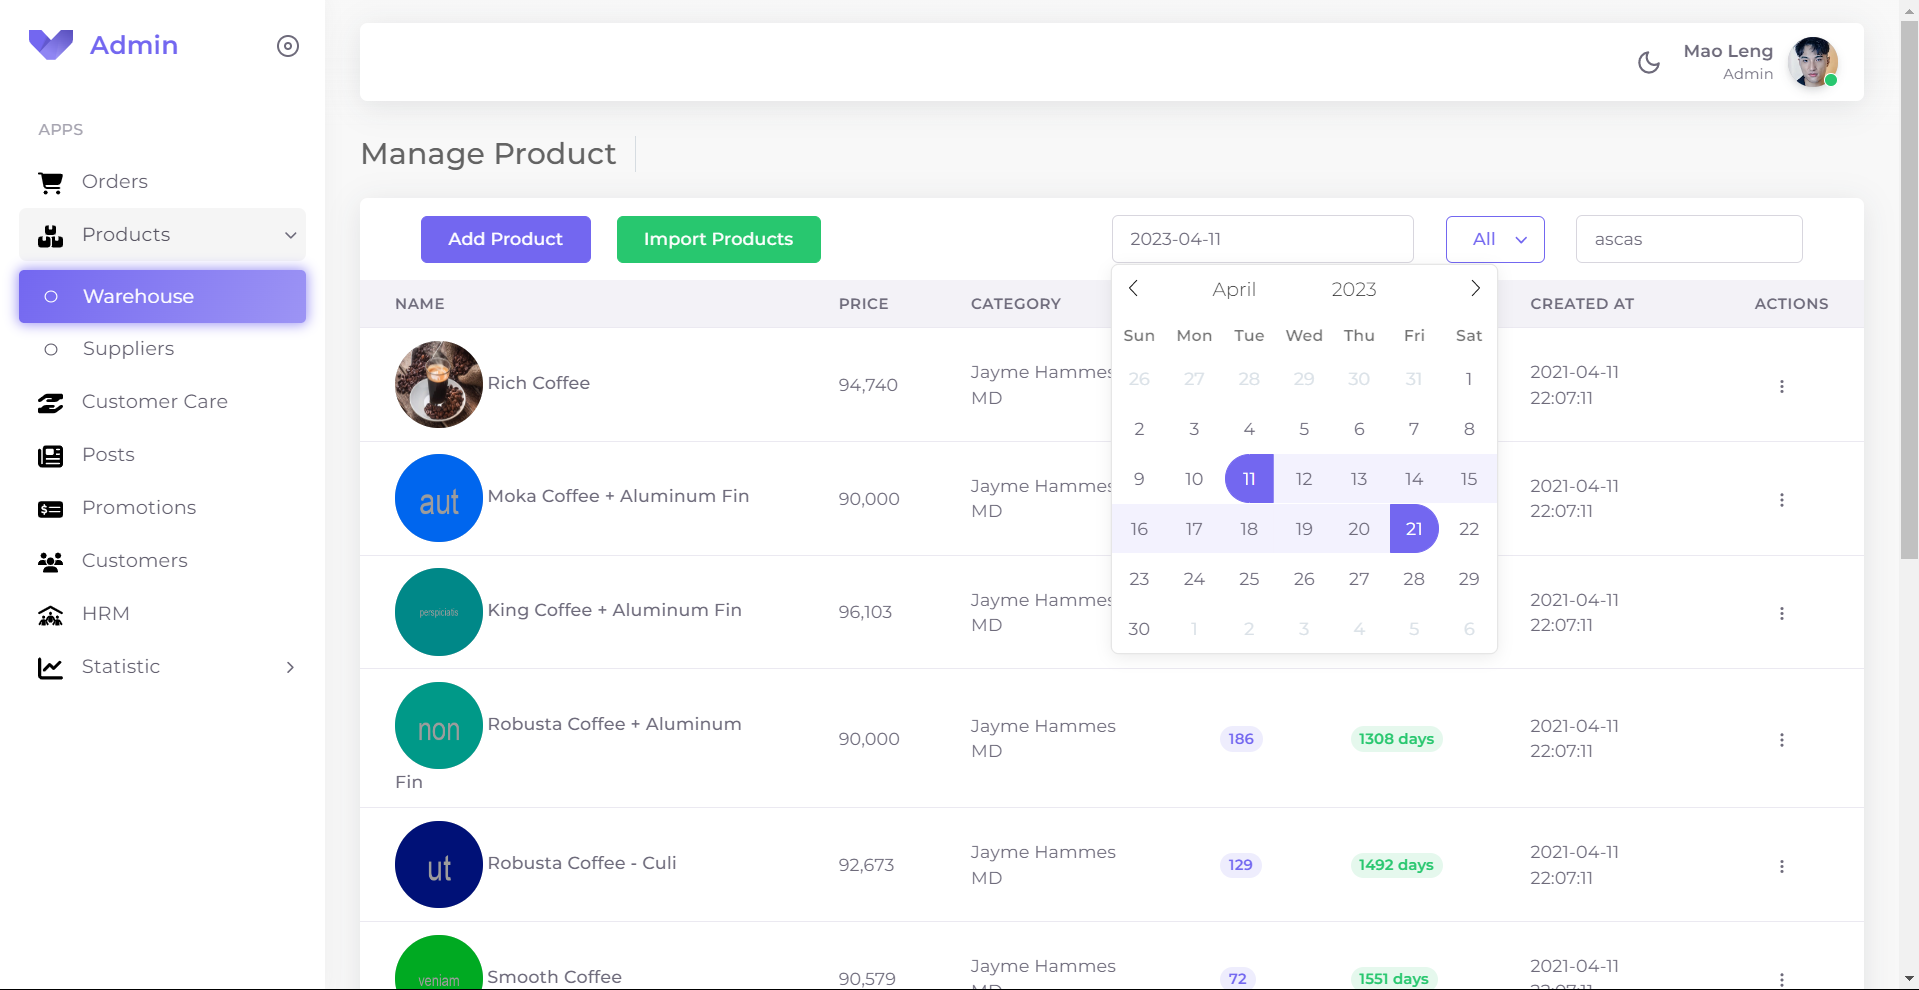
\includegraphics[width=0.7\textwidth]{Demo/Screenshot_10.png}
    \label{fig:supportpage}
\end{figure}
\begin{figure}[H]
    \centering
    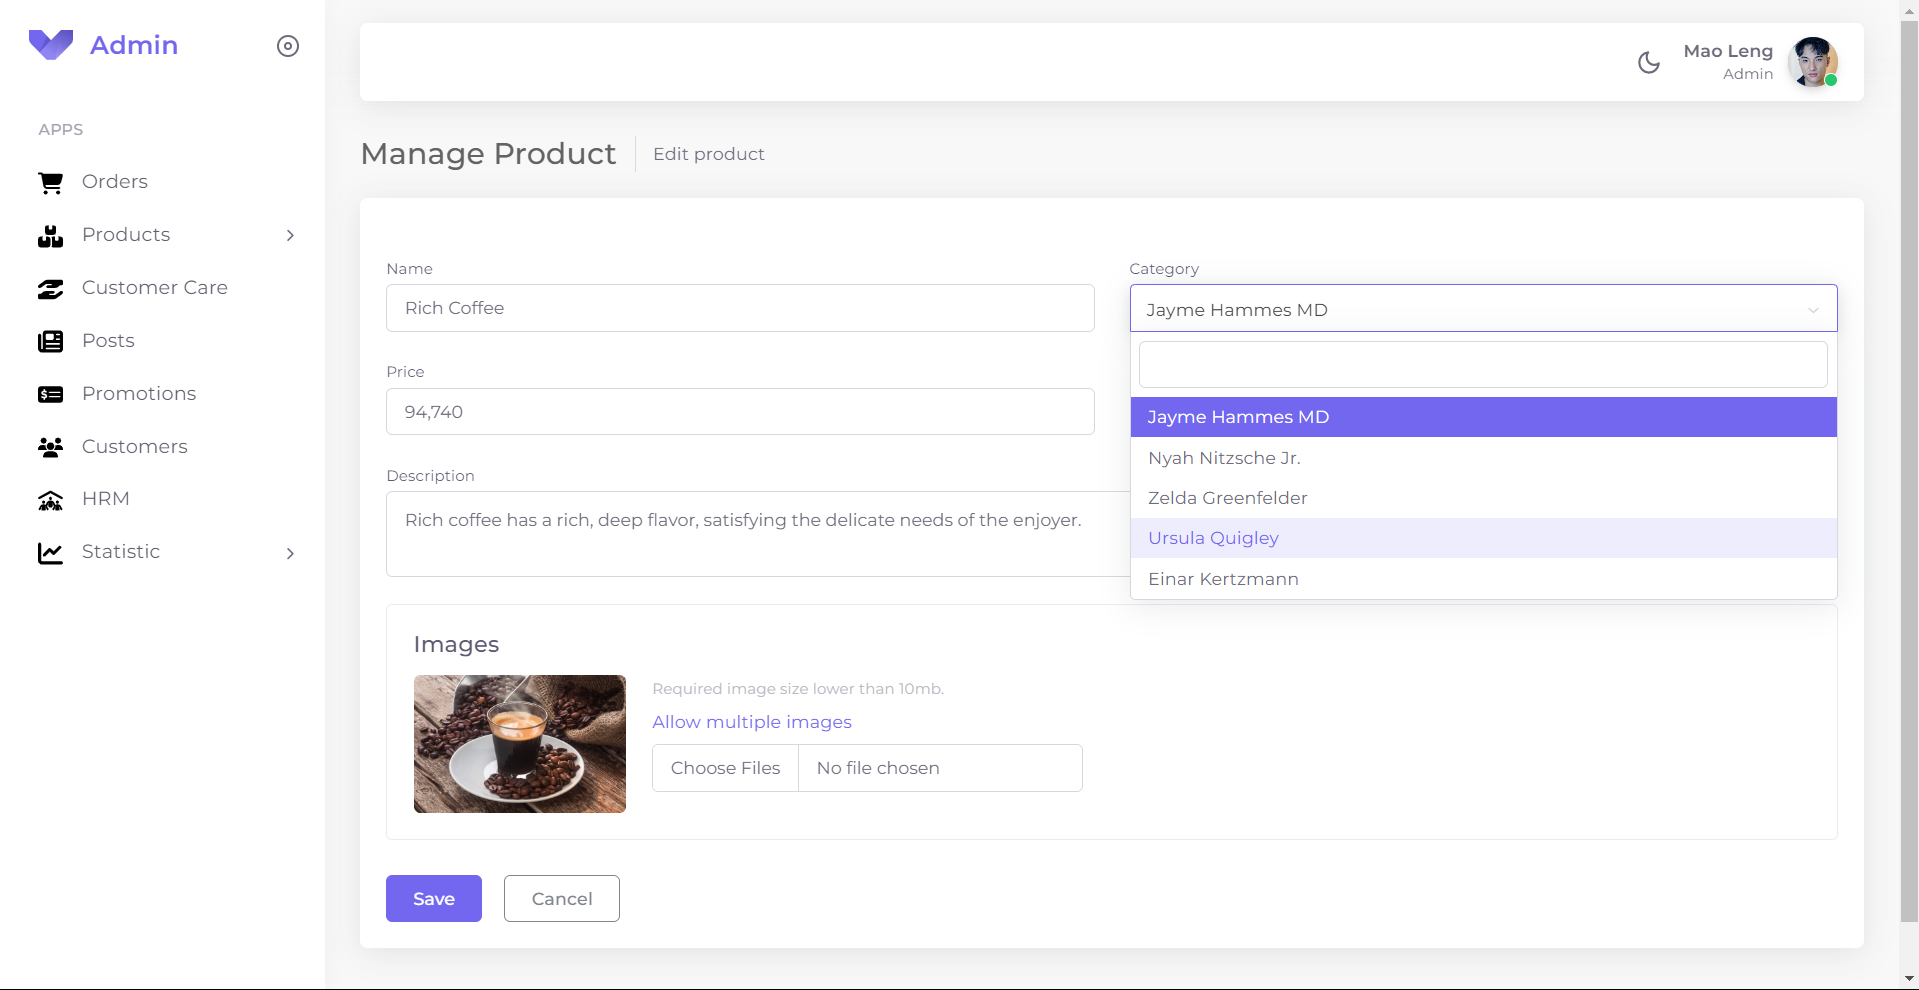
\includegraphics[width=0.7\textwidth]{Demo/Screenshot_11.png}
    \label{fig:supportpage}
\end{figure}
\begin{figure}[H]
    \centering
    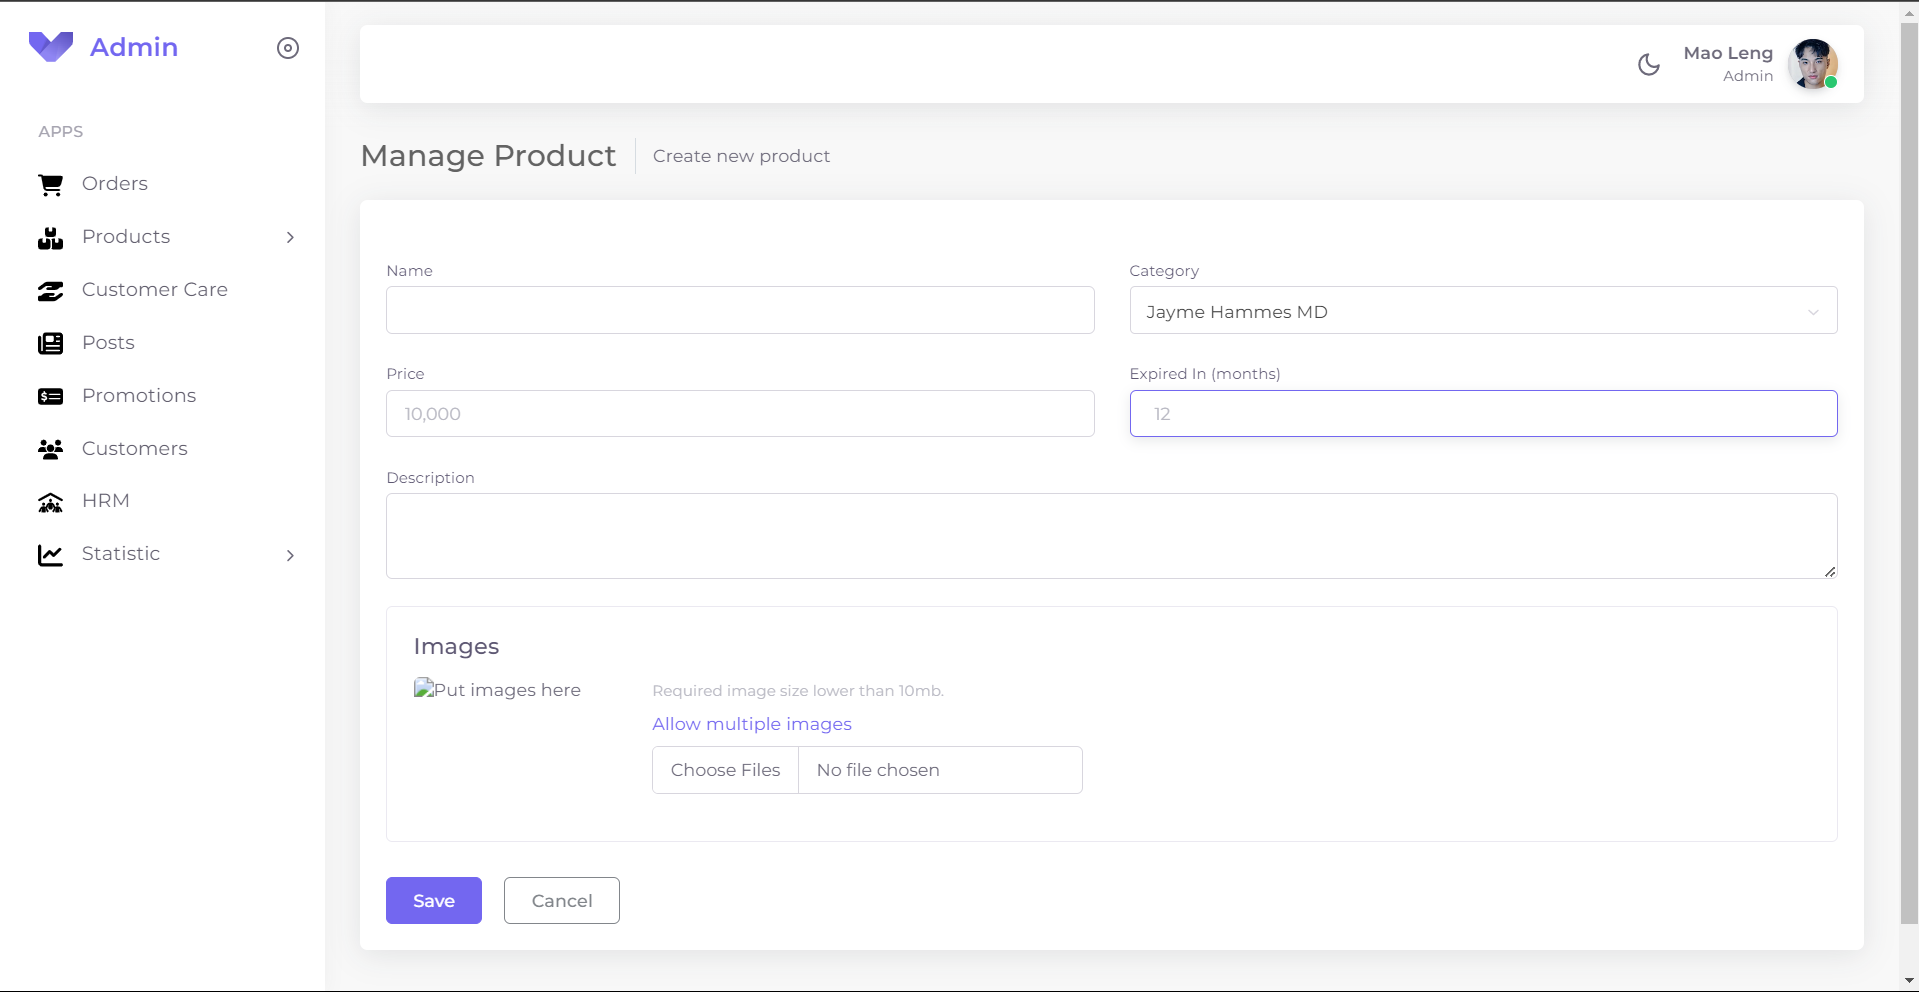
\includegraphics[width=0.7\textwidth]{Demo/Screenshot_12.png}
    \label{fig:supportpage}
\end{figure}
\begin{figure}[H]
    \centering
    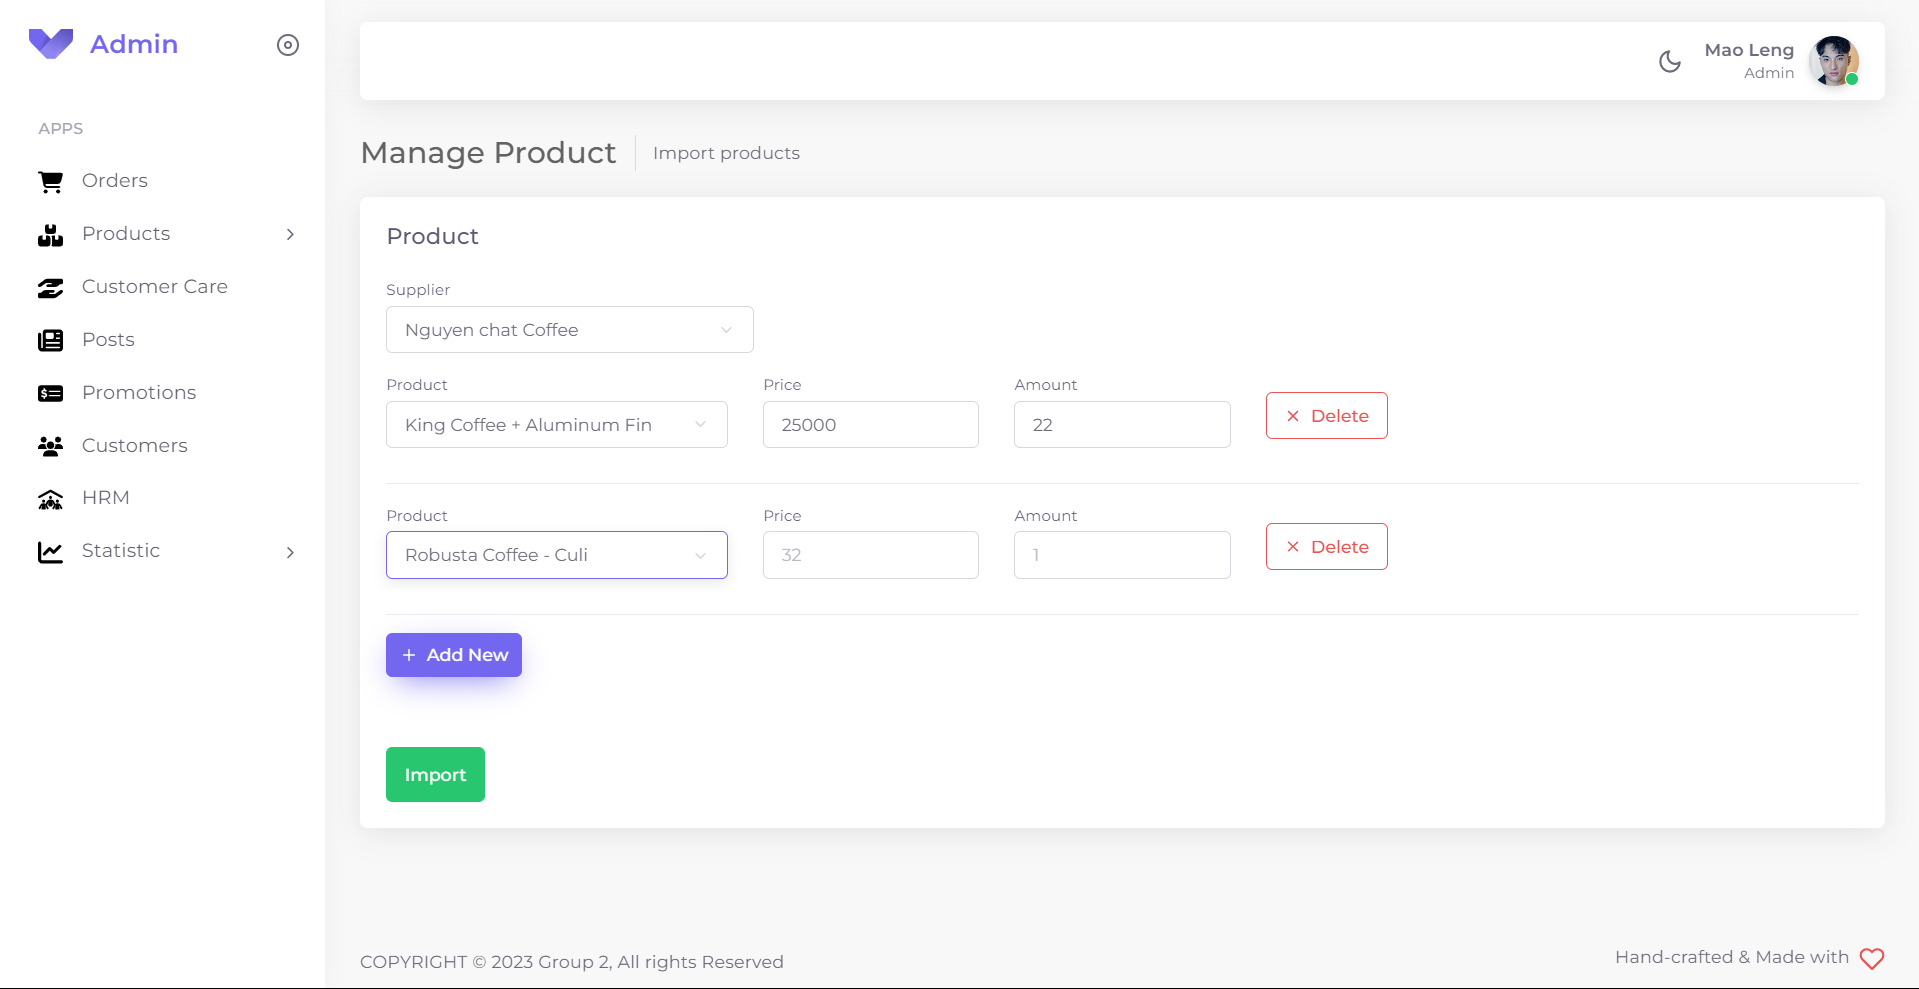
\includegraphics[width=0.7\textwidth]{Demo/Screenshot_13.png}
    \label{fig:supportpage}
\end{figure}

\subsection{Manage post}
1. Login first \\
2. User navigates to the website's Manage post at \href{https://coffee.skrt.cc/admin/post}{here}. \\
3. User can search by input, filter by time range, filter by category\\
4. User can edit post's information by clicking edit button, fill the new data, then click save.\\
5. User can store post's information by clicking Add new post button, fill the data, then click save.\\
6. User can delete post by clicking Delete.\\
\begin{figure}[H]
    \centering
    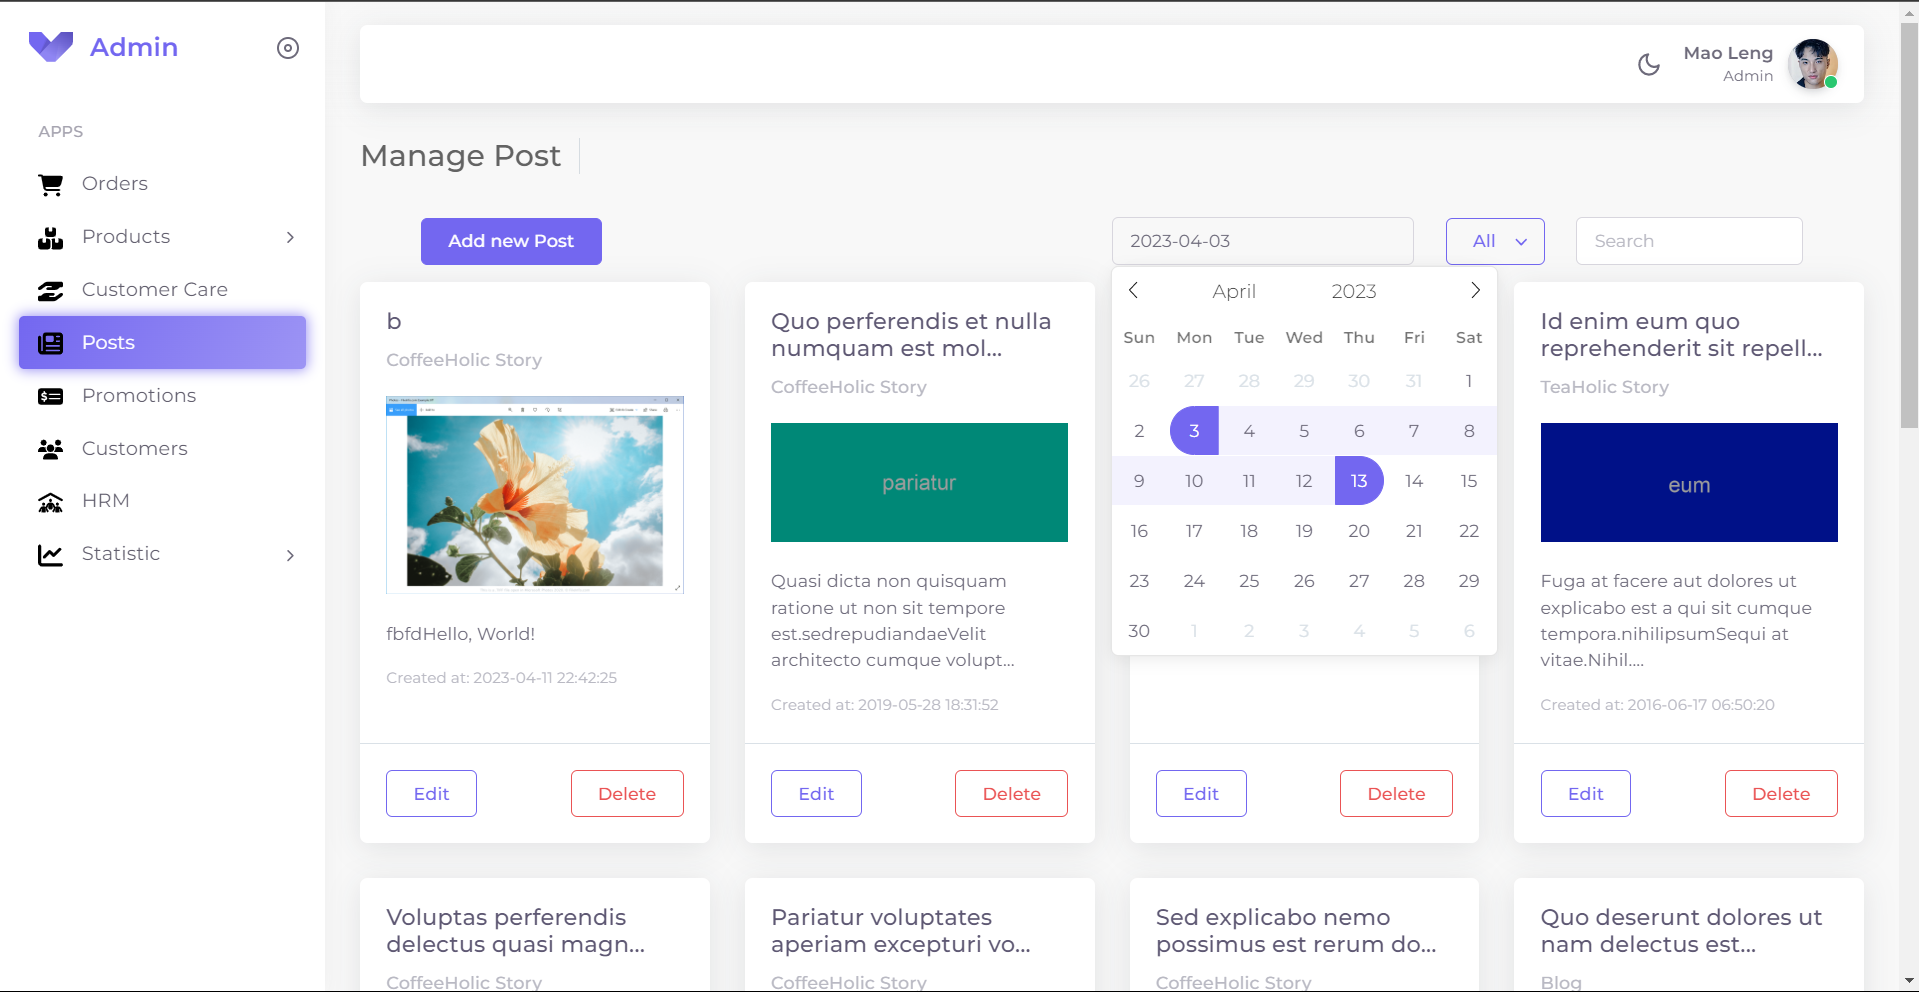
\includegraphics[width=0.7\textwidth]{Demo/Screenshot_14.png}
    \label{fig:supportpage}
\end{figure}
\begin{figure}[H]
    \centering
    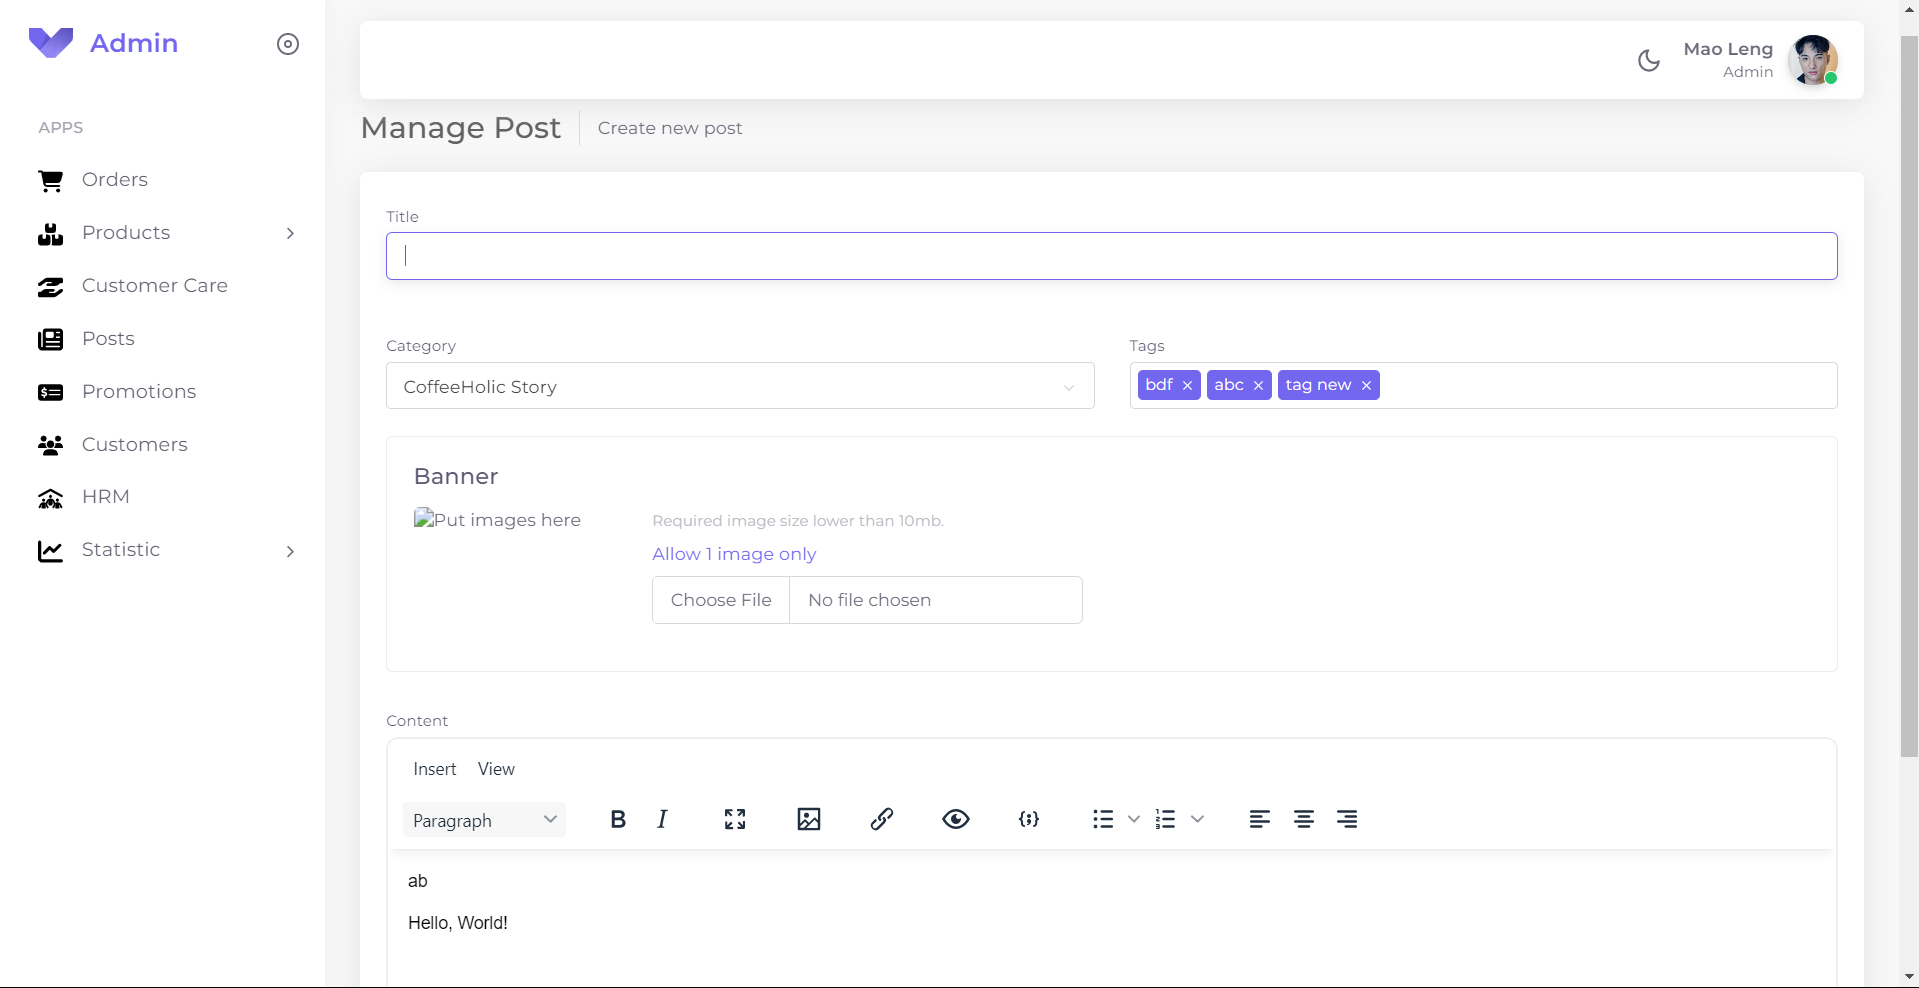
\includegraphics[width=0.7\textwidth]{Demo/Screenshot_15.png}
    \label{fig:supportpage}
\end{figure}
\begin{figure}[H]
    \centering
    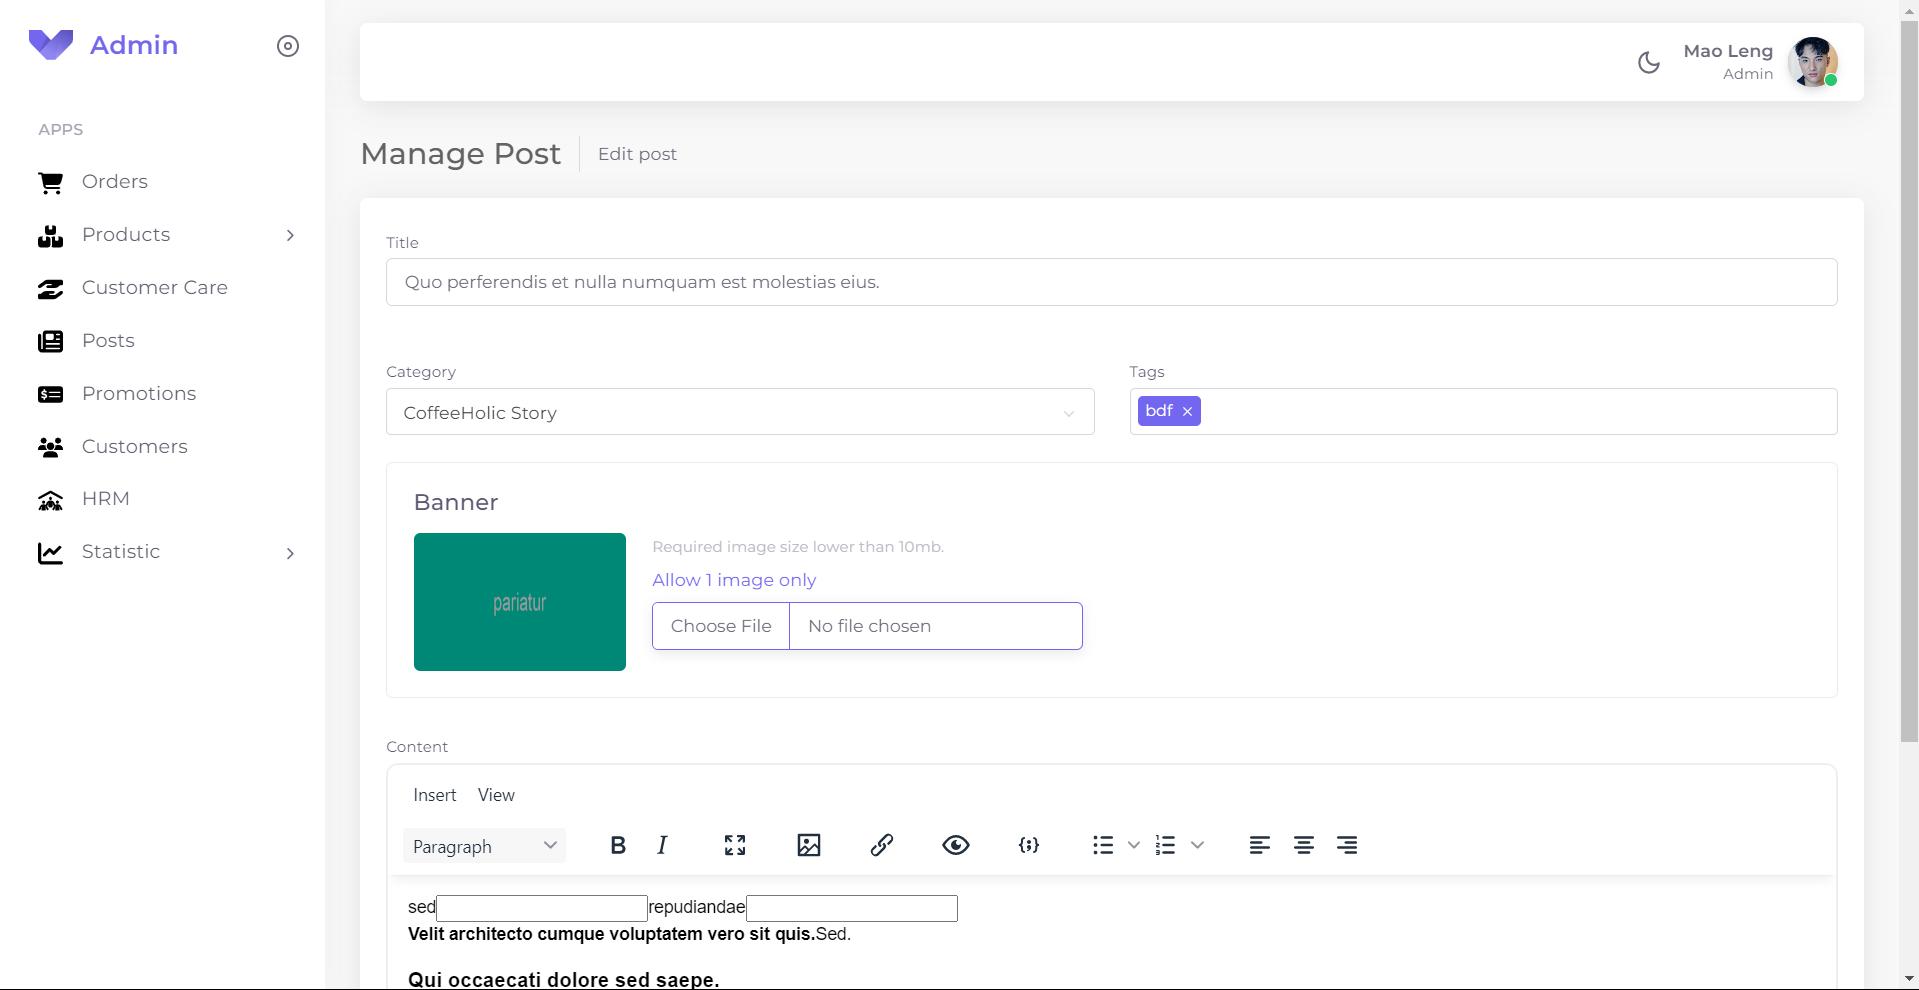
\includegraphics[width=0.7\textwidth]{Demo/Screenshot_16.png}
    \label{fig:supportpage}
\end{figure}

\subsection{Manage promotion}
1. Login first \\
2. User navigates to the website's Manage promotion and repository at \href{https://coffee.skrt.cc/admin/promotion}{here}. \\
3. User can search by input, filter by time range, filter by status\\
4. User can edit promotion's information by clicking edit button, fill the new data, then click save.\\
5. User can store promotion's information by clicking Add new promotion button, fill the data, then click save.\\
\begin{figure}[H]
    \centering
    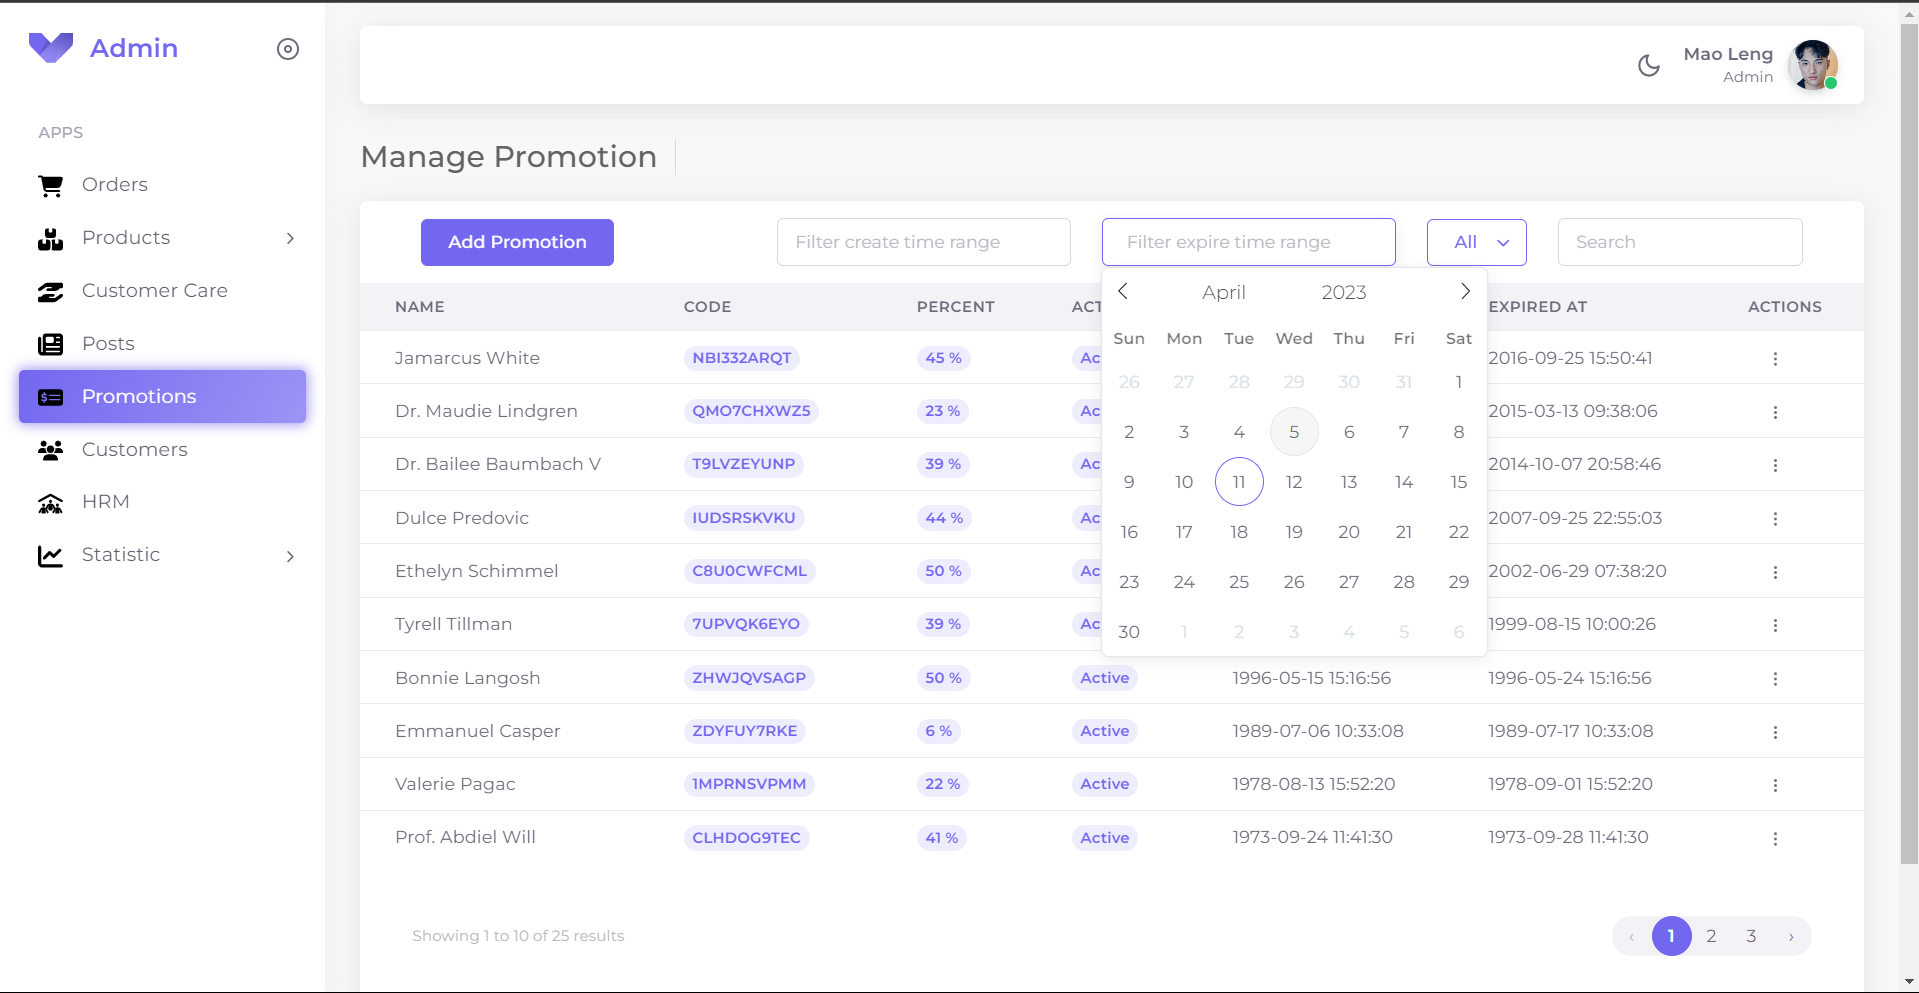
\includegraphics[width=0.7\textwidth]{Demo/Screenshot_17.png}
    \label{fig:supportpage}
\end{figure}
\begin{figure}[H]
    \centering
    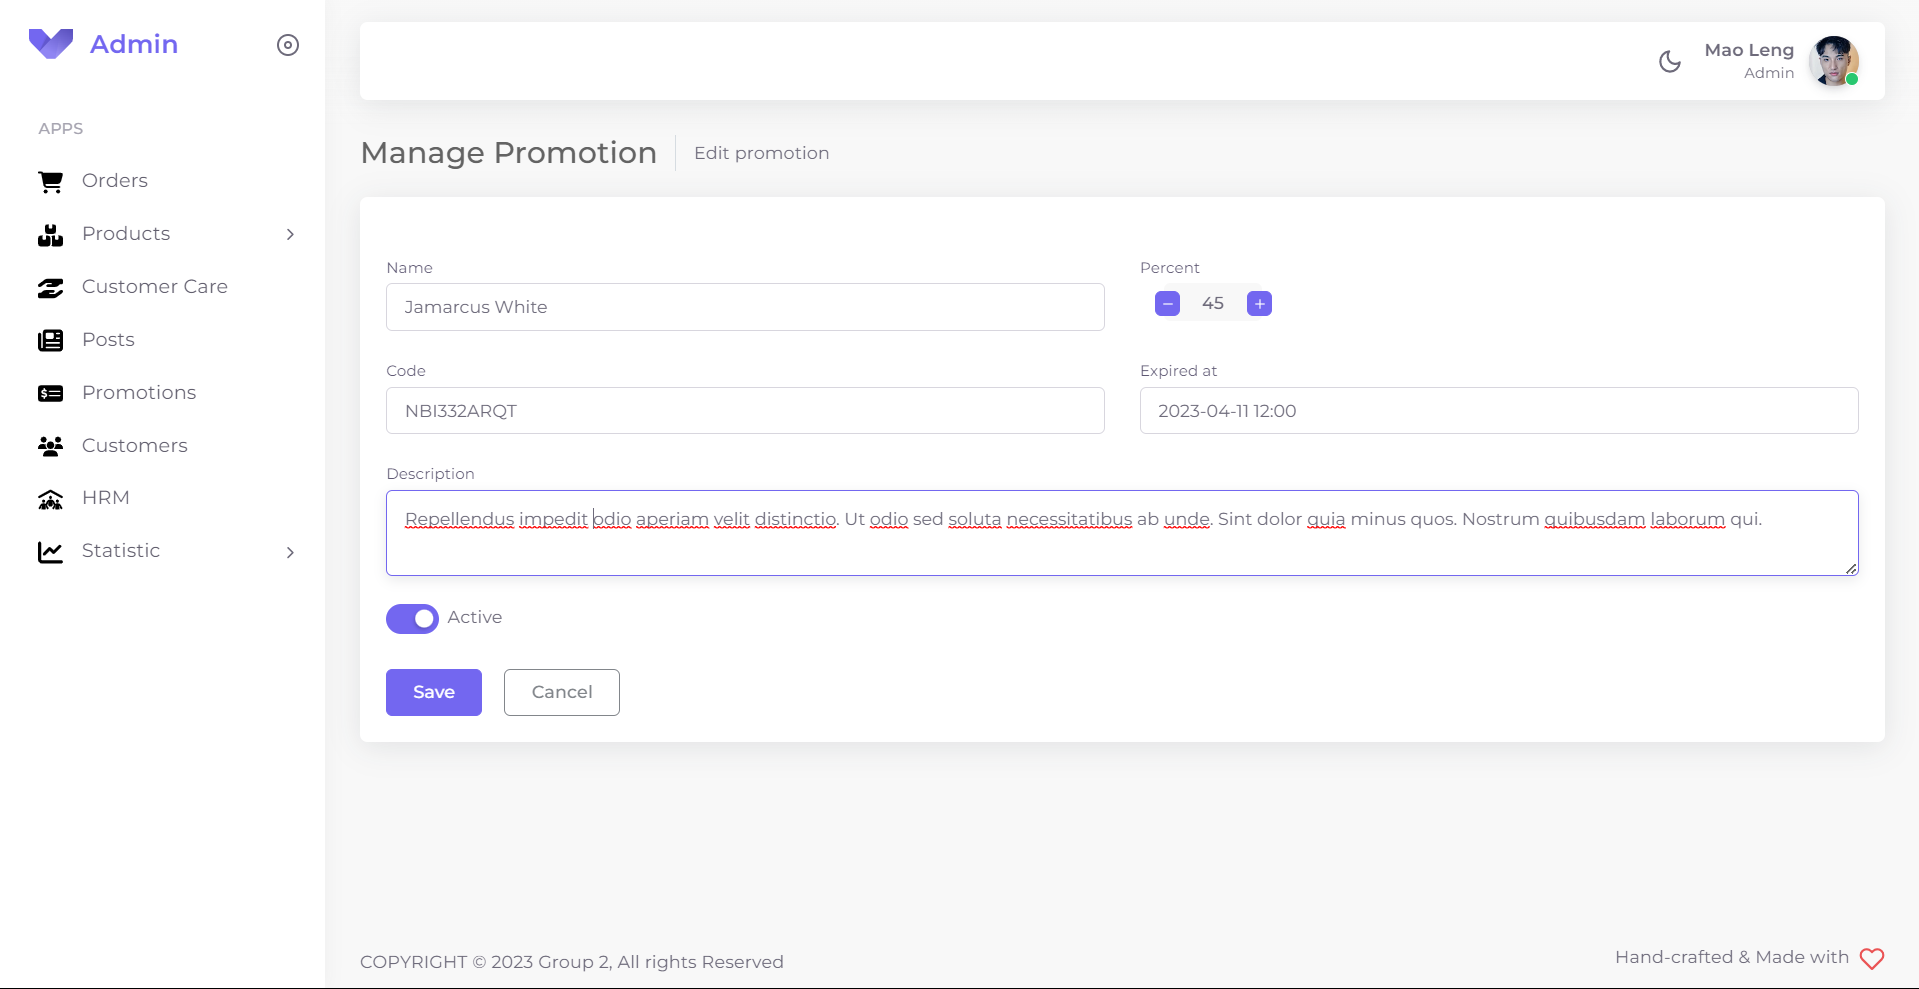
\includegraphics[width=0.7\textwidth]{Demo/Screenshot_18.png}
    \label{fig:supportpage}
\end{figure}
\begin{figure}[H]
    \centering
    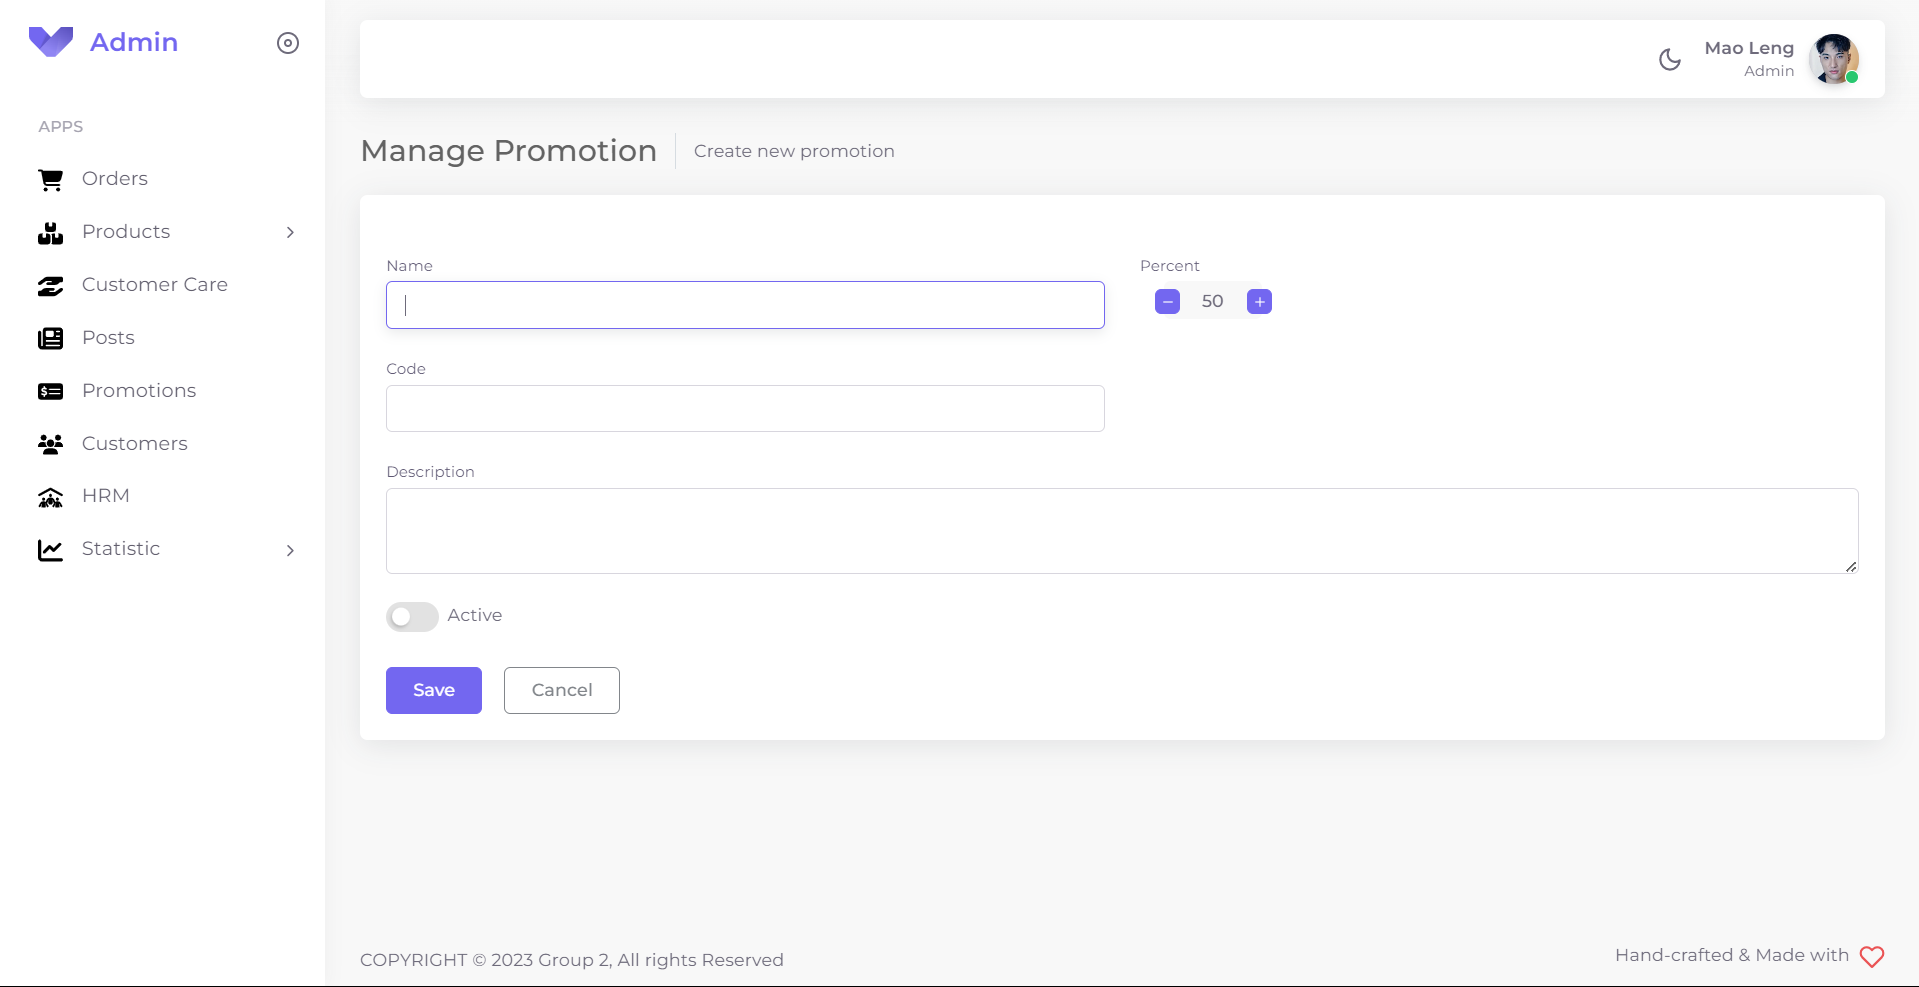
\includegraphics[width=0.7\textwidth]{Demo/Screenshot_19.png}
    \label{fig:supportpage}
\end{figure}

\subsection{Manage order}
1. Login first \\
2. User navigates to the website's Manage order and repository at \href{https://coffee.skrt.cc/admin/order}{here}. \\
3. User can search by input, filter by time range, filter by status\\
4. User can approve or decline the order, check which order is paid already, change status of the order.\\
5. User can see order detail and print the bill.\\

\begin{figure}[H]
    \centering
    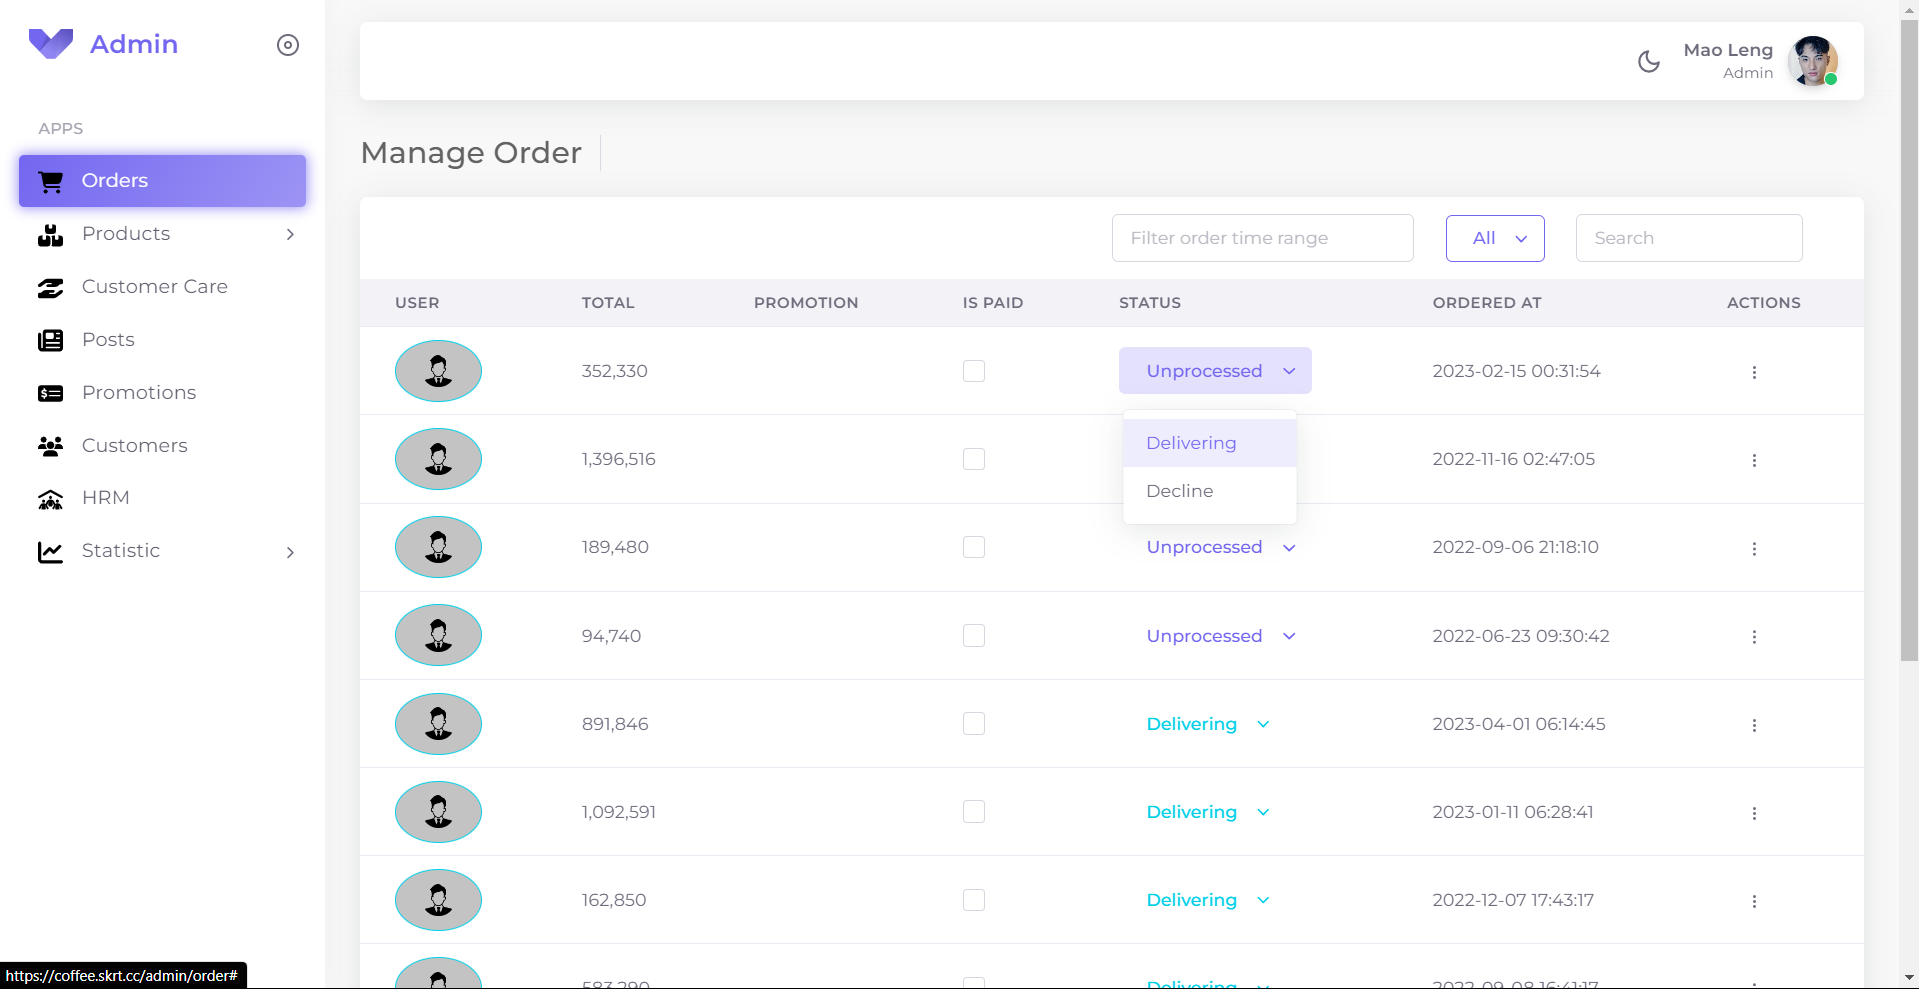
\includegraphics[width=0.7\textwidth]{Demo/Screenshot_22.png}
    \label{fig:supportpage}
\end{figure}
\begin{figure}[H]
    \centering
    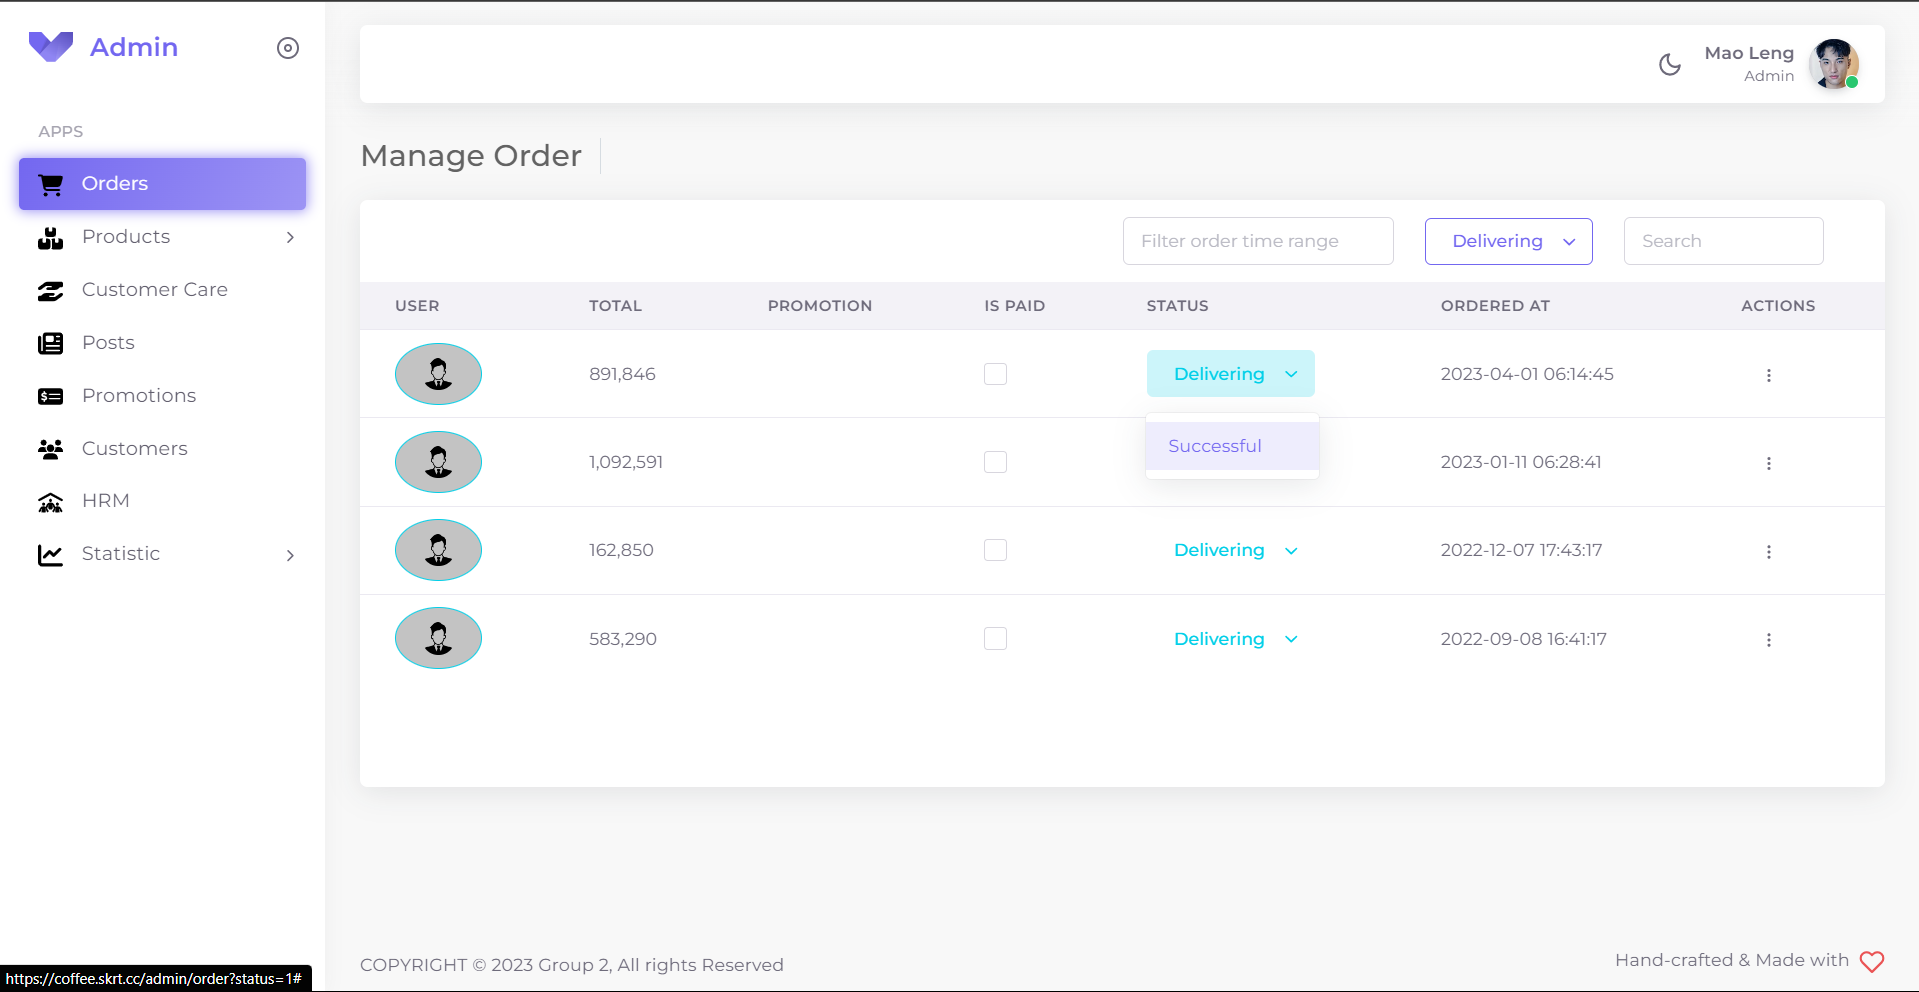
\includegraphics[width=0.7\textwidth]{Demo/Screenshot_23.png}
    \label{fig:supportpage}
\end{figure}
\begin{figure}[H]
    \centering
    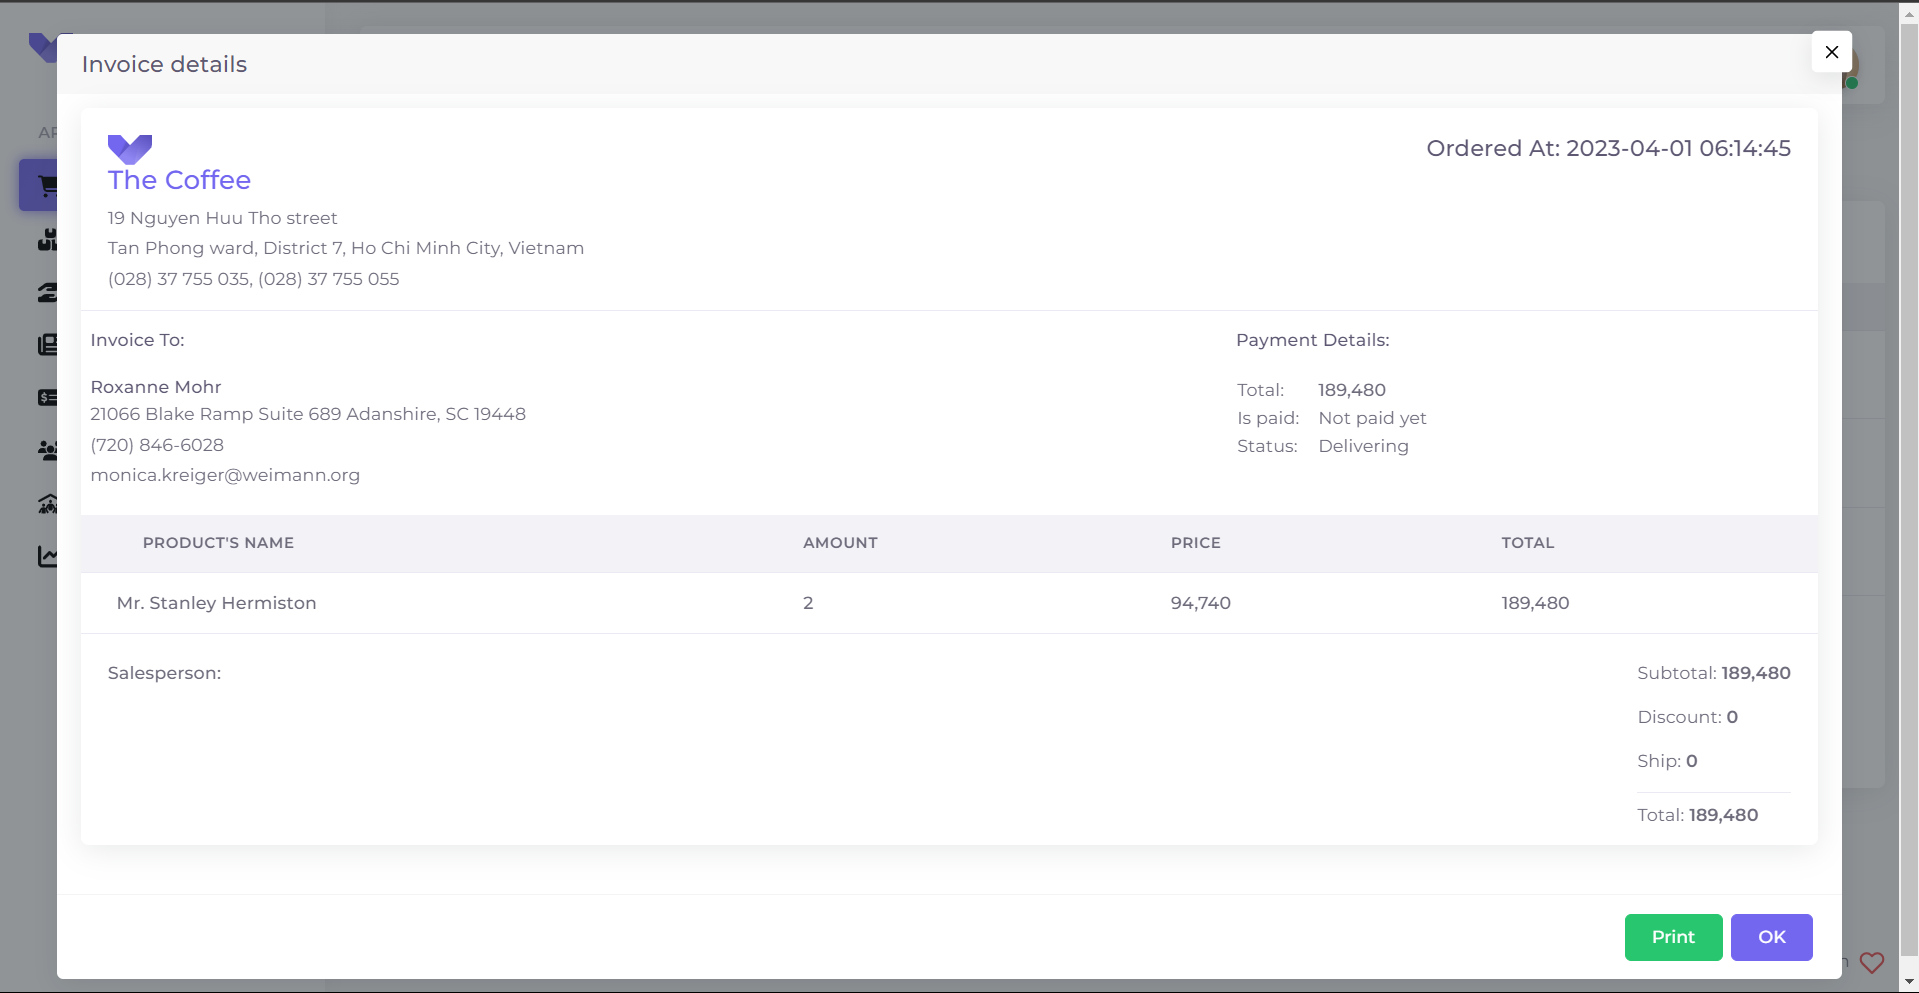
\includegraphics[width=0.7\textwidth]{Demo/Screenshot_24.png}
    \label{fig:supportpage}
\end{figure}

\subsection{Manage Customer Care}
1. Login first \\
2. User navigates to the website's Customer Care at \href{https://coffee.skrt.cc/admin/customer-care}{here}. \\
3. User can search by input, filter by time range, filter by status\\
4. User can reply to the request by clicking Response on the action, then fill the content and press Send.\\
5. User can filter the request.\\
\begin{figure}[H]
    \centering
    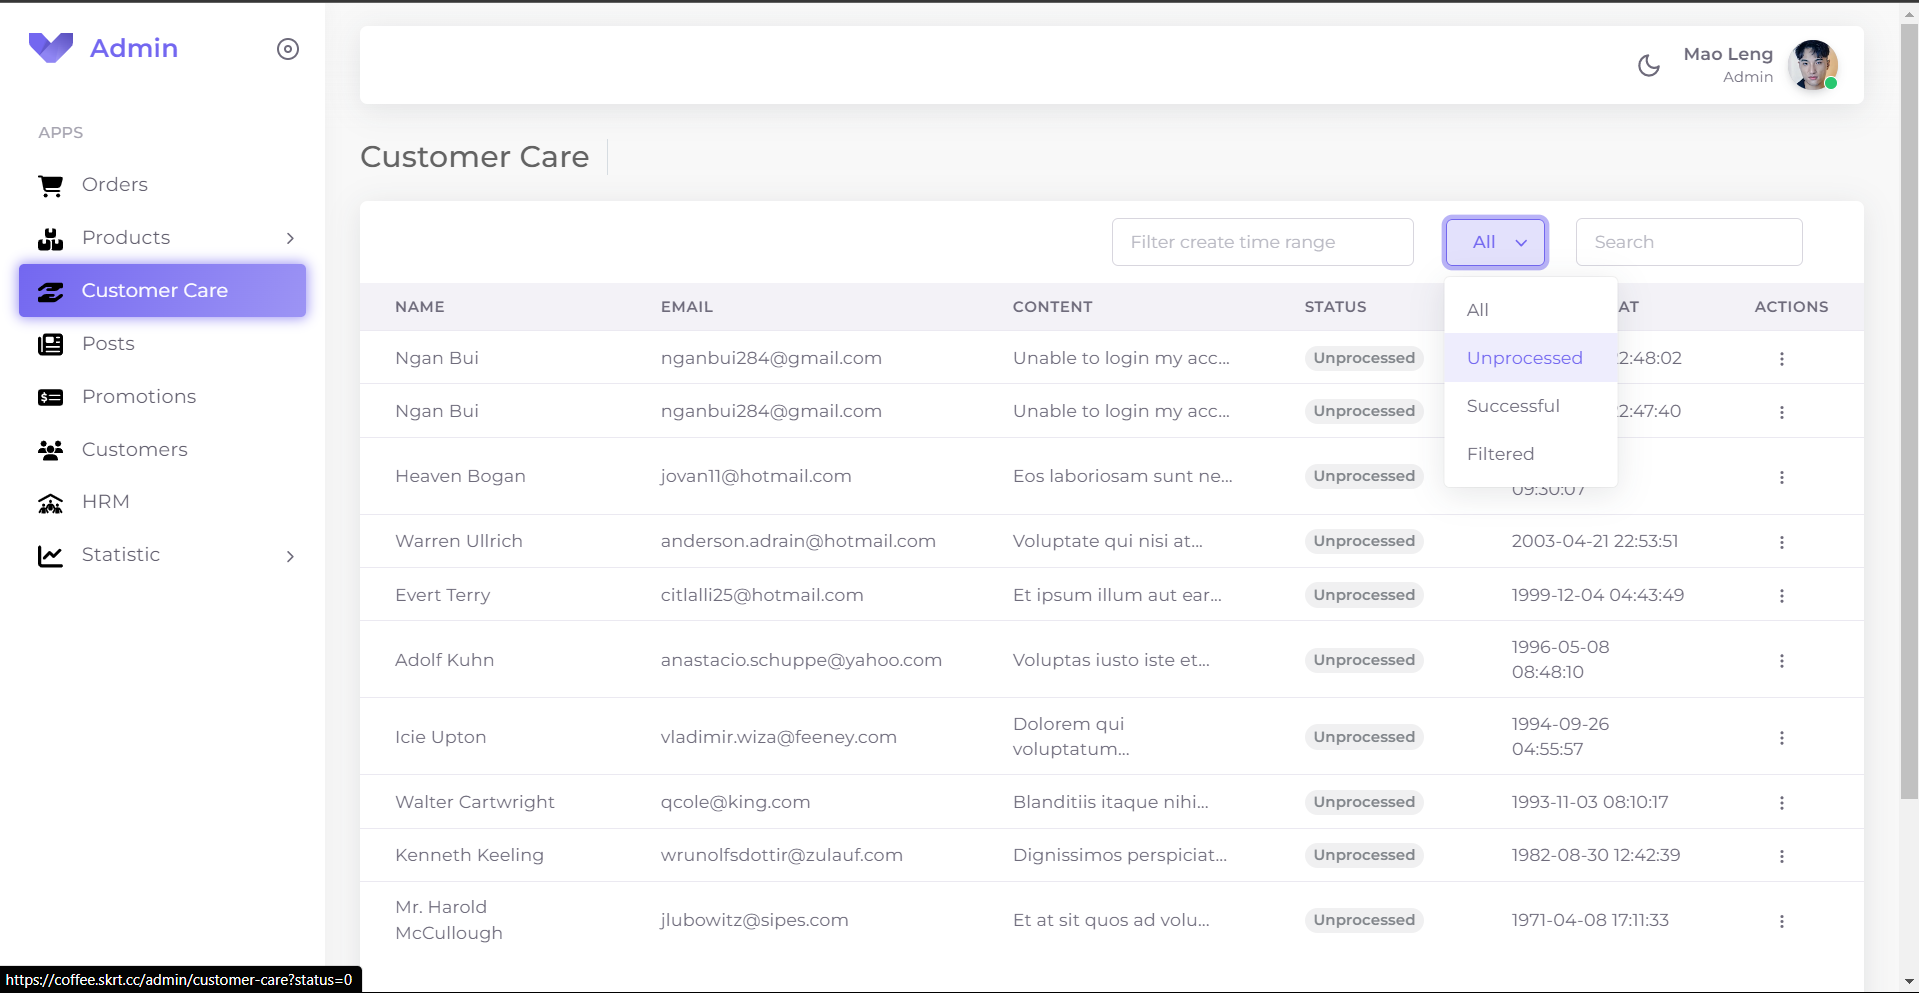
\includegraphics[width=0.7\textwidth]{Demo/Screenshot_20.png}
    \label{fig:supportpage}
\end{figure}
\begin{figure}[H]
    \centering
    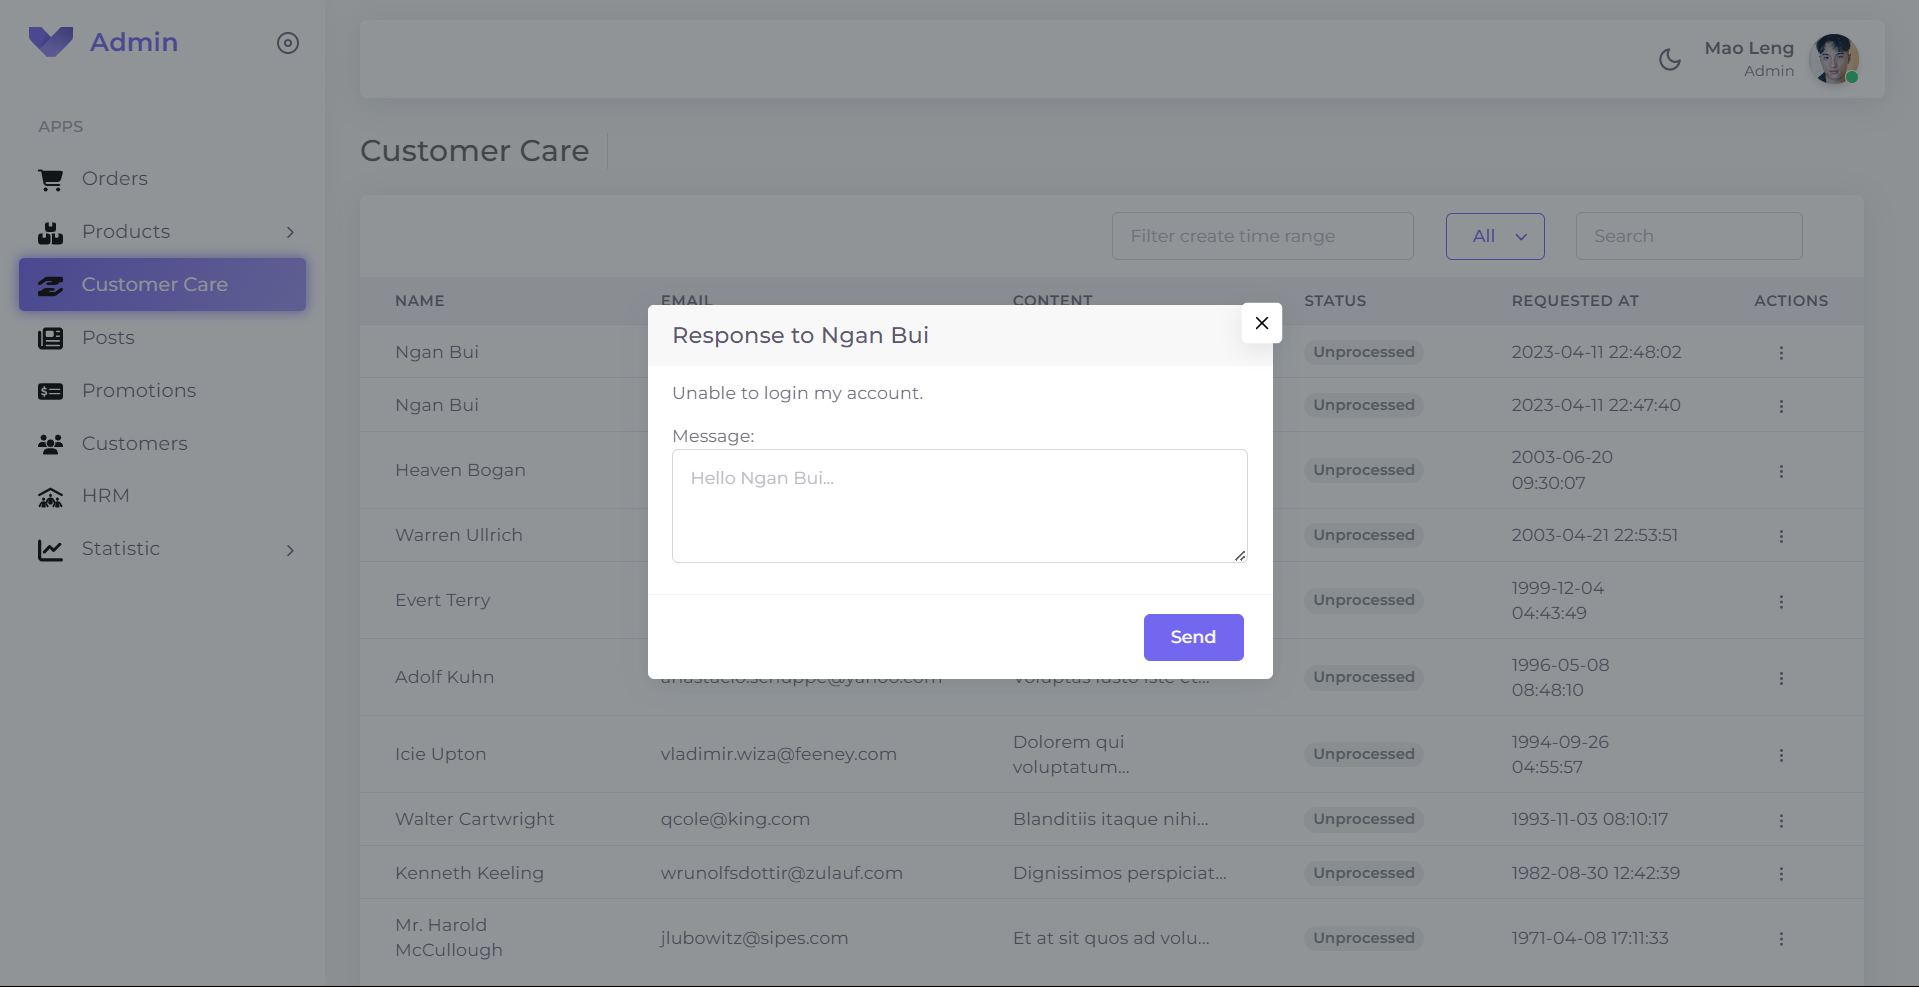
\includegraphics[width=0.7\textwidth]{Demo/Screenshot_21.png}
    \label{fig:supportpage}
\end{figure}

\subsection{Send a support request}
1. User navigates to the website's product page at \href{https://coffee.skrt.cc/support}{here}. \\
\begin{figure}[H]
    \centering
    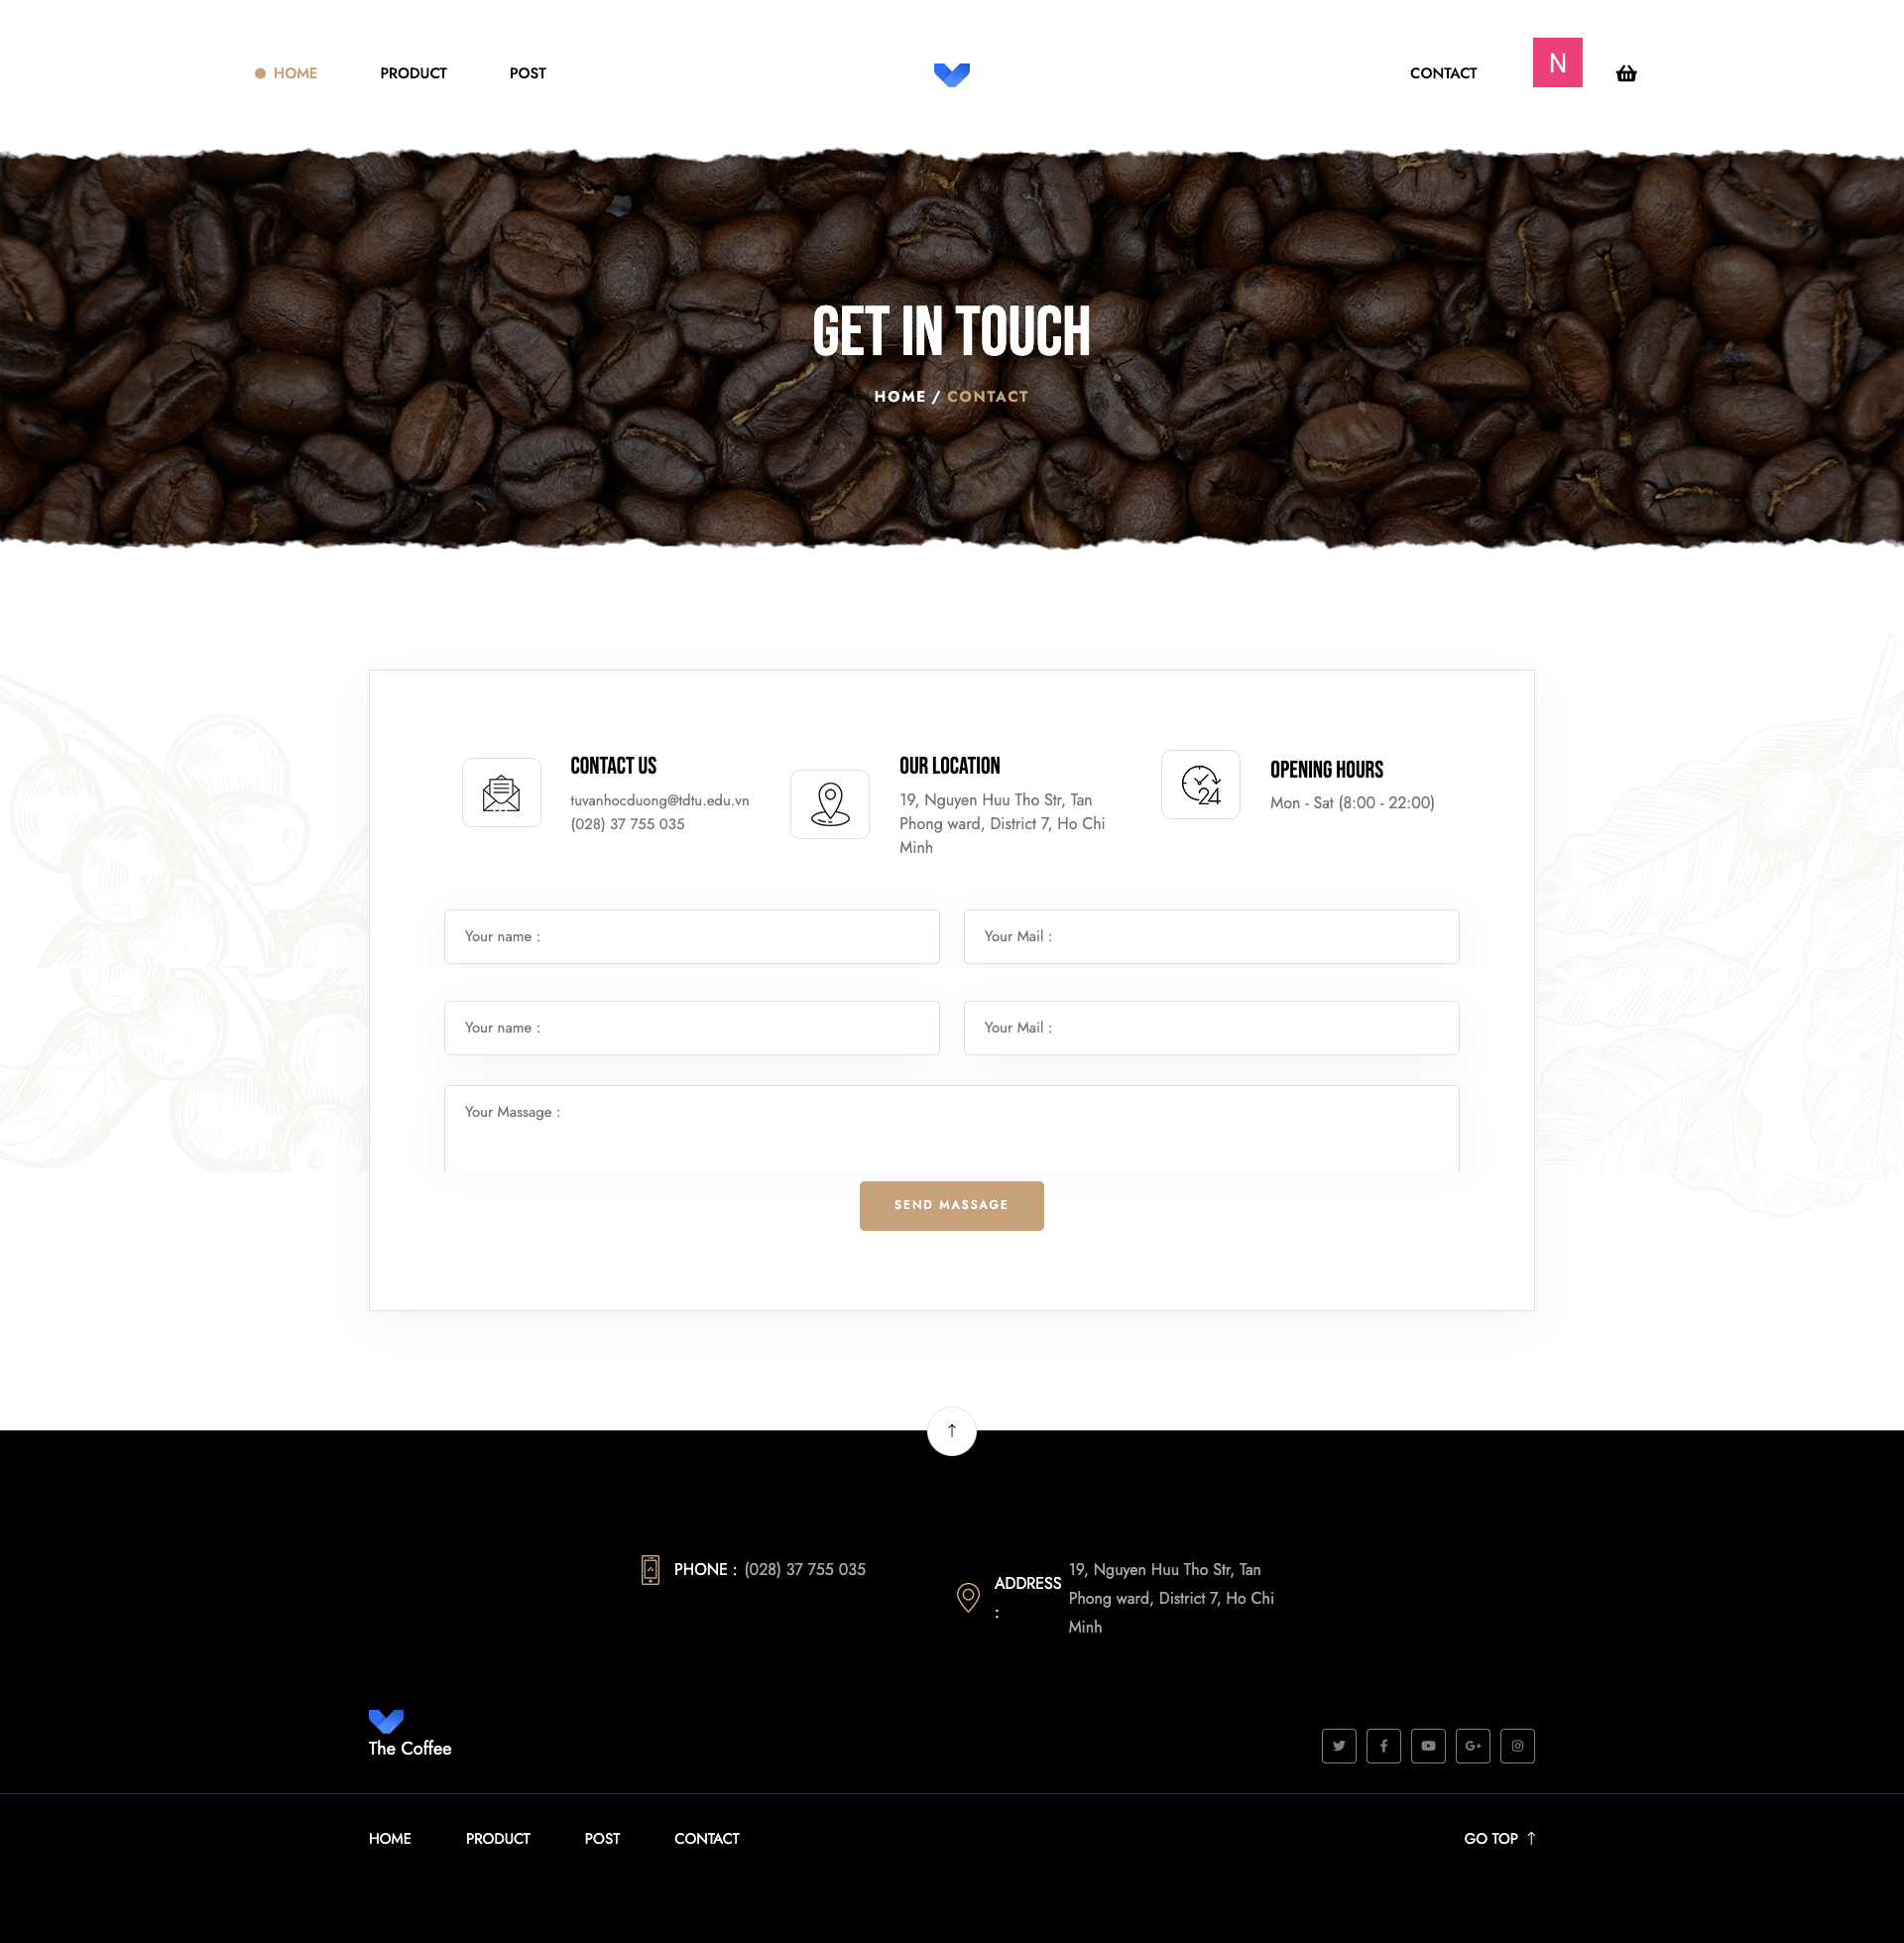
\includegraphics[width=0.7\textwidth]{Demo/SupportPage.png}
    \label{fig:supportpage}
\end{figure}
2. User can enter name, email and description. After finish, they enter "Send Message" to send request. Then, the system will announce the result.
\subsection{Search/View product}
1. The user navigates to the website's product page at \href{https://coffee.skrt.cc/}{here}. \\
2. The user browses the different coffee products.\\
\begin{figure}[H]
    \centering
    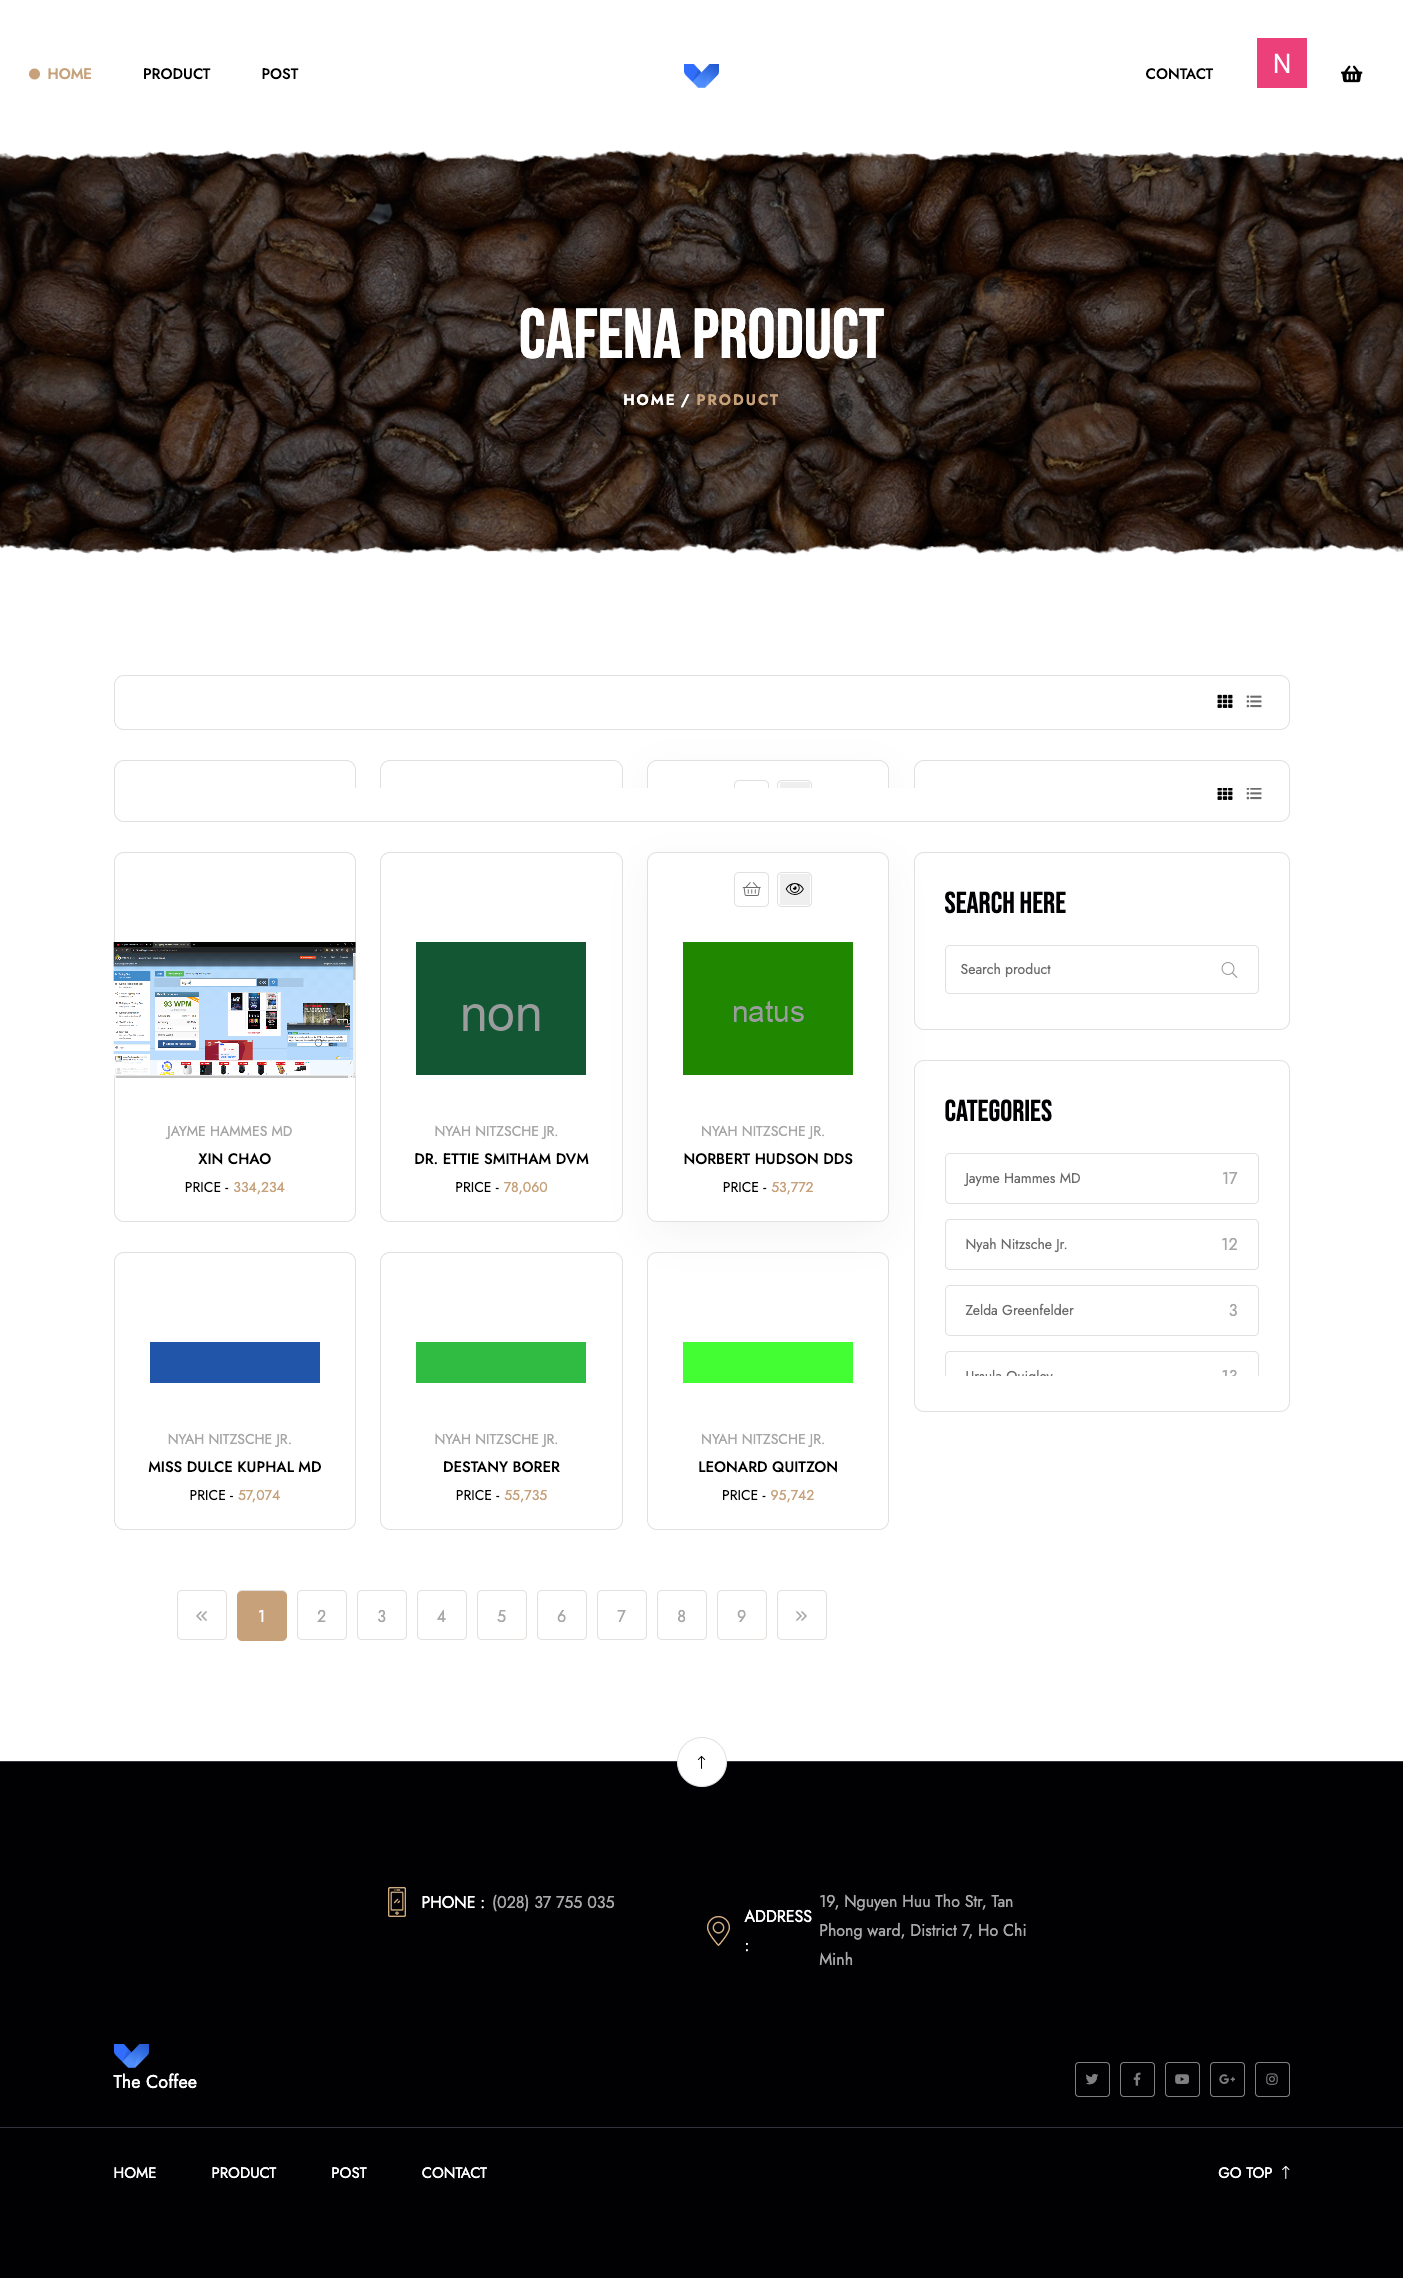
\includegraphics[width=0.7\textwidth]{Demo/Product.png}
    \label{fig:productpage}
\end{figure}
3. The user clicks on a specific coffee product to view its details and add it to their cart. The website loads the coffee product details on a new page, including its image, name, description, price, and related products. \\
\subsection{Manage cart}
1. The user clicks on the cart icon to add the coffee product to their cart. \\
2. The website adds the coffee product to the user's cart, updates the cart icon and the cart total, and displays a confirmation message. \\
3. The user clicks on the cart icon to view their cart and check out. \\
4. The website loads the cart page, displaying a list of the coffee products in the cart, their quantities, prices, and the total price. \\
5. The user reviews the cart details and clicks on the "Proceed to checkout" button.
\begin{figure}[H]
    \centering
    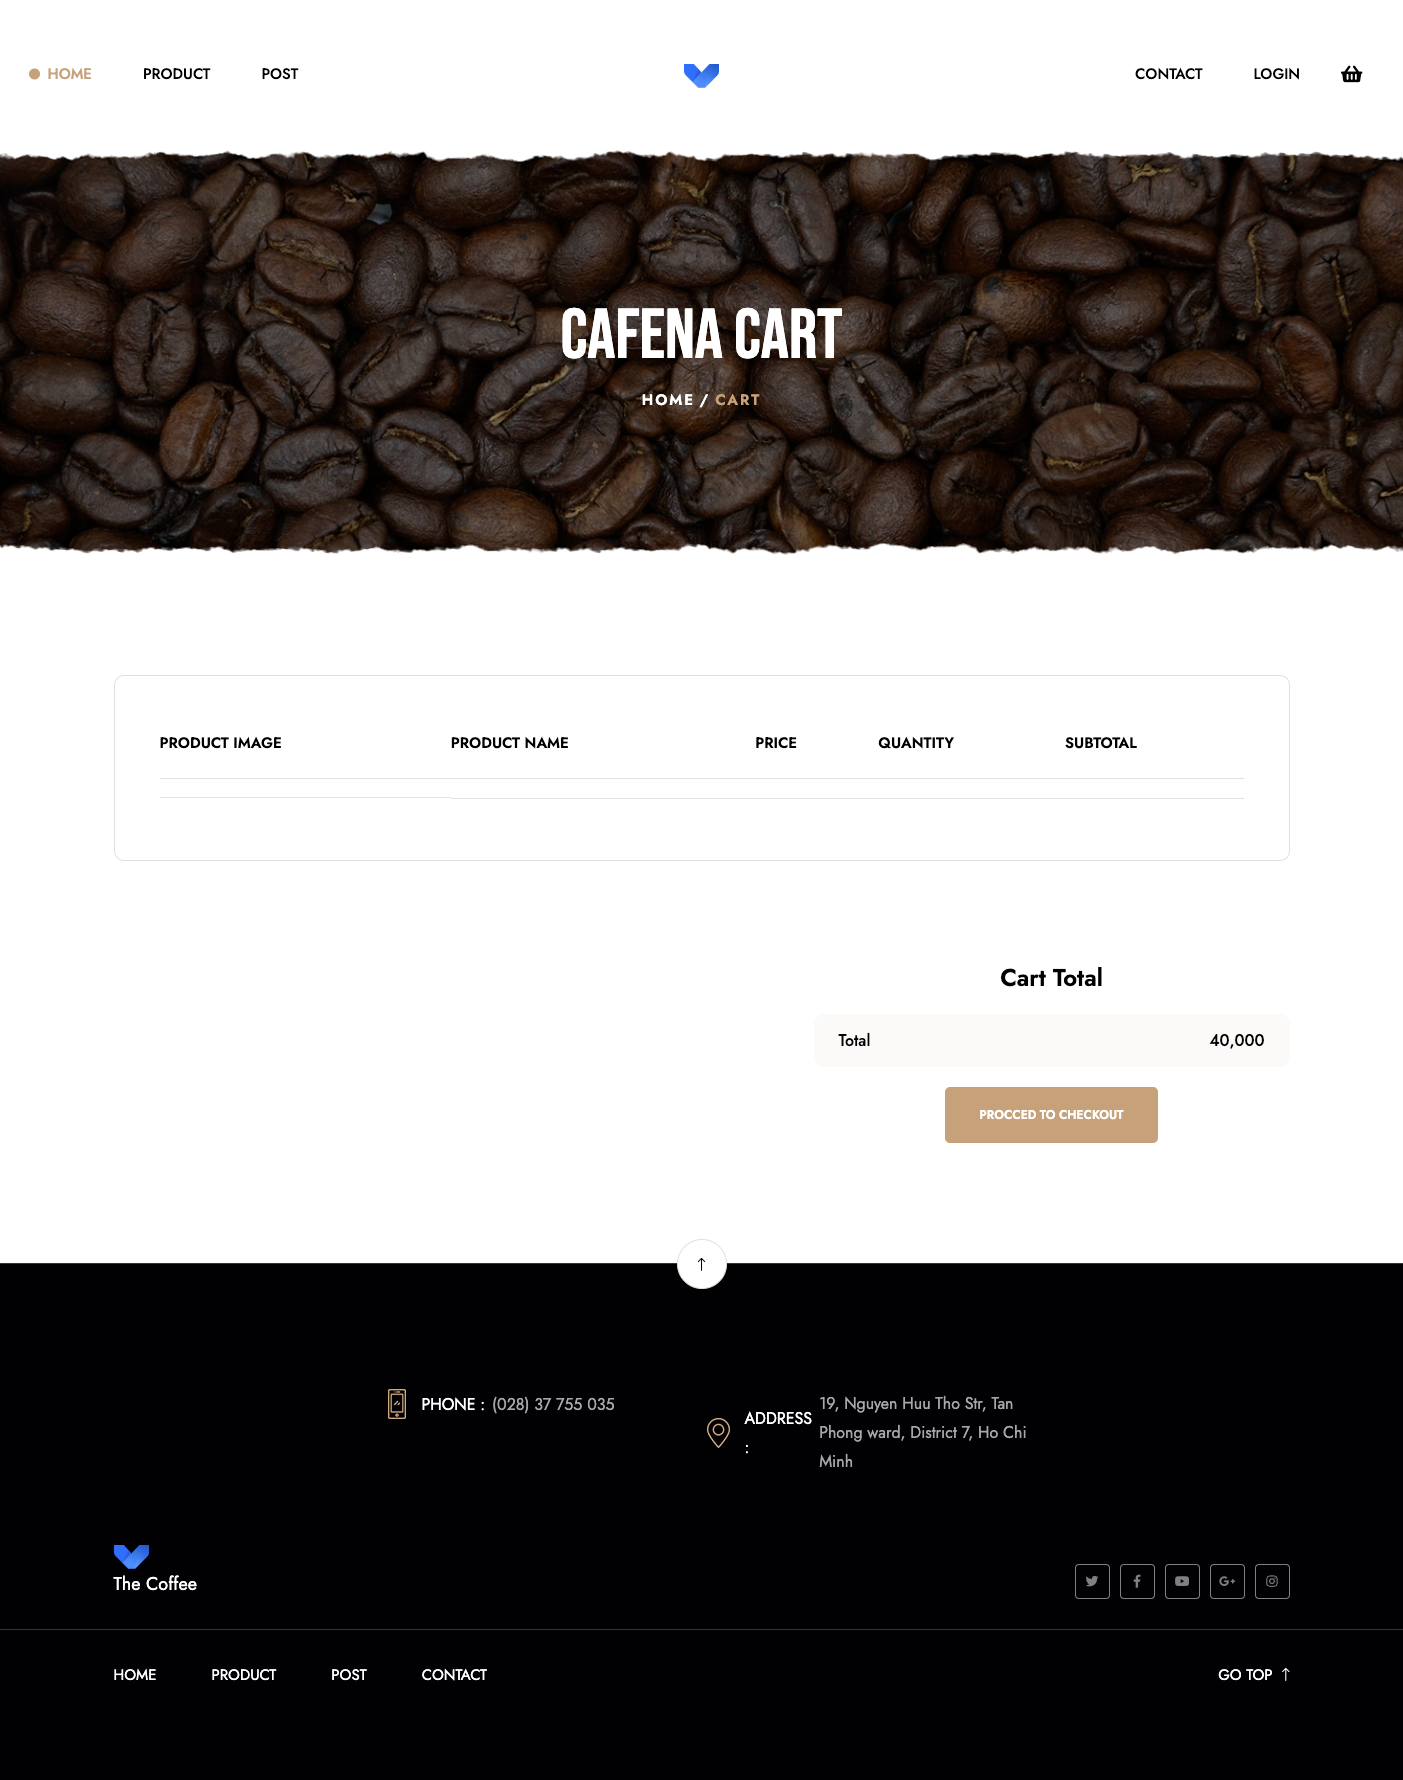
\includegraphics[width=0.7\textwidth]{Demo/Cart.png}
    \label{fig:cartpage}
\end{figure}
\subsection{Order}
1. The website loads the checkout page, displaying a form for the user to enter their shipping and payment information. \\
\begin{figure}[H]
    \centering
    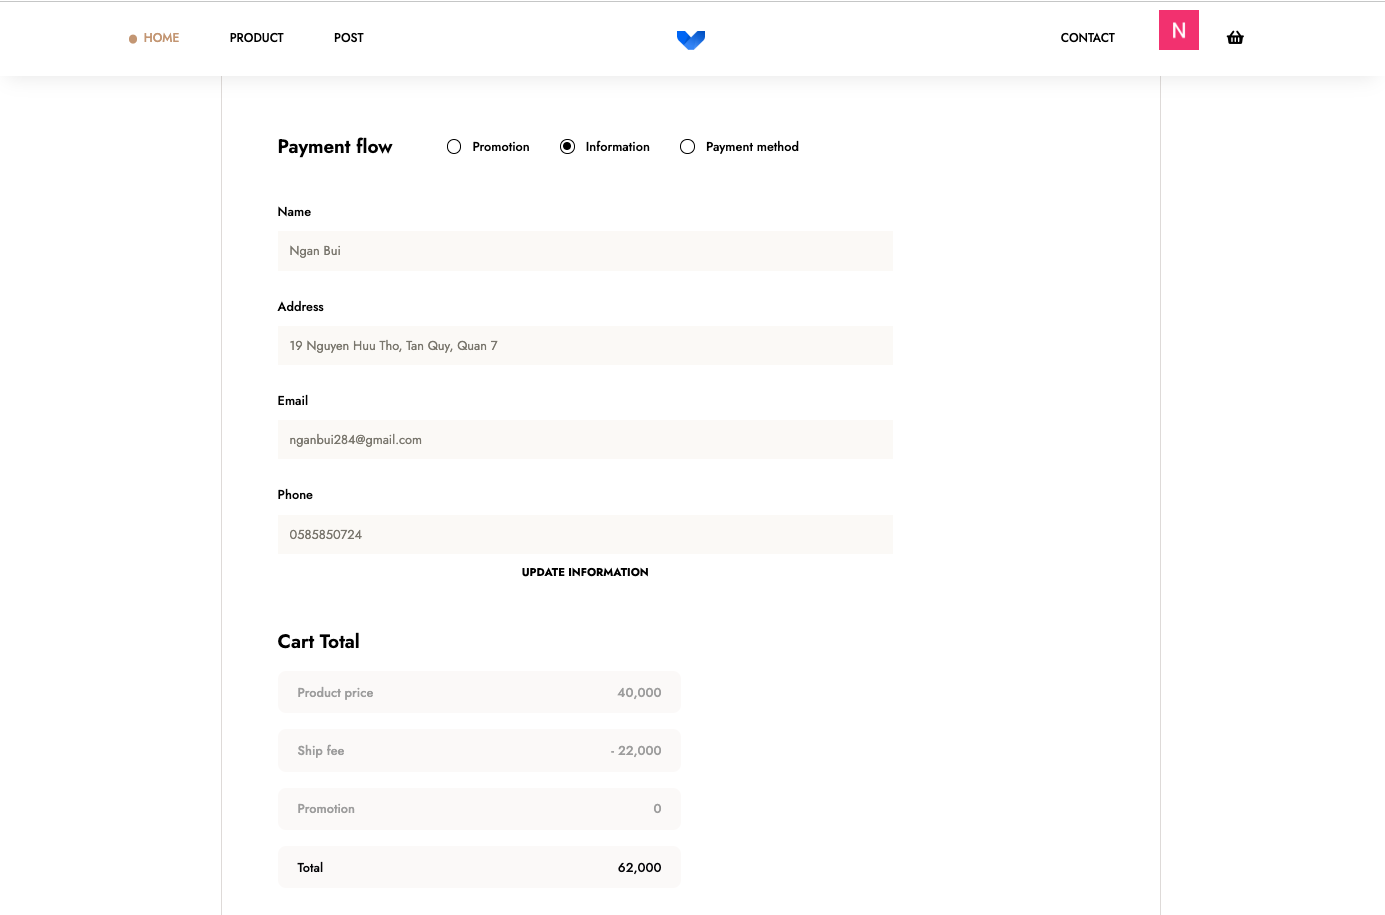
\includegraphics[width=0.7\textwidth]{Demo/Cart1.png}
    \label{fig:cart1page}
\end{figure}
2. The user fills out the checkout form and go to "Payment Method". 
\begin{figure}[H]
    \centering
    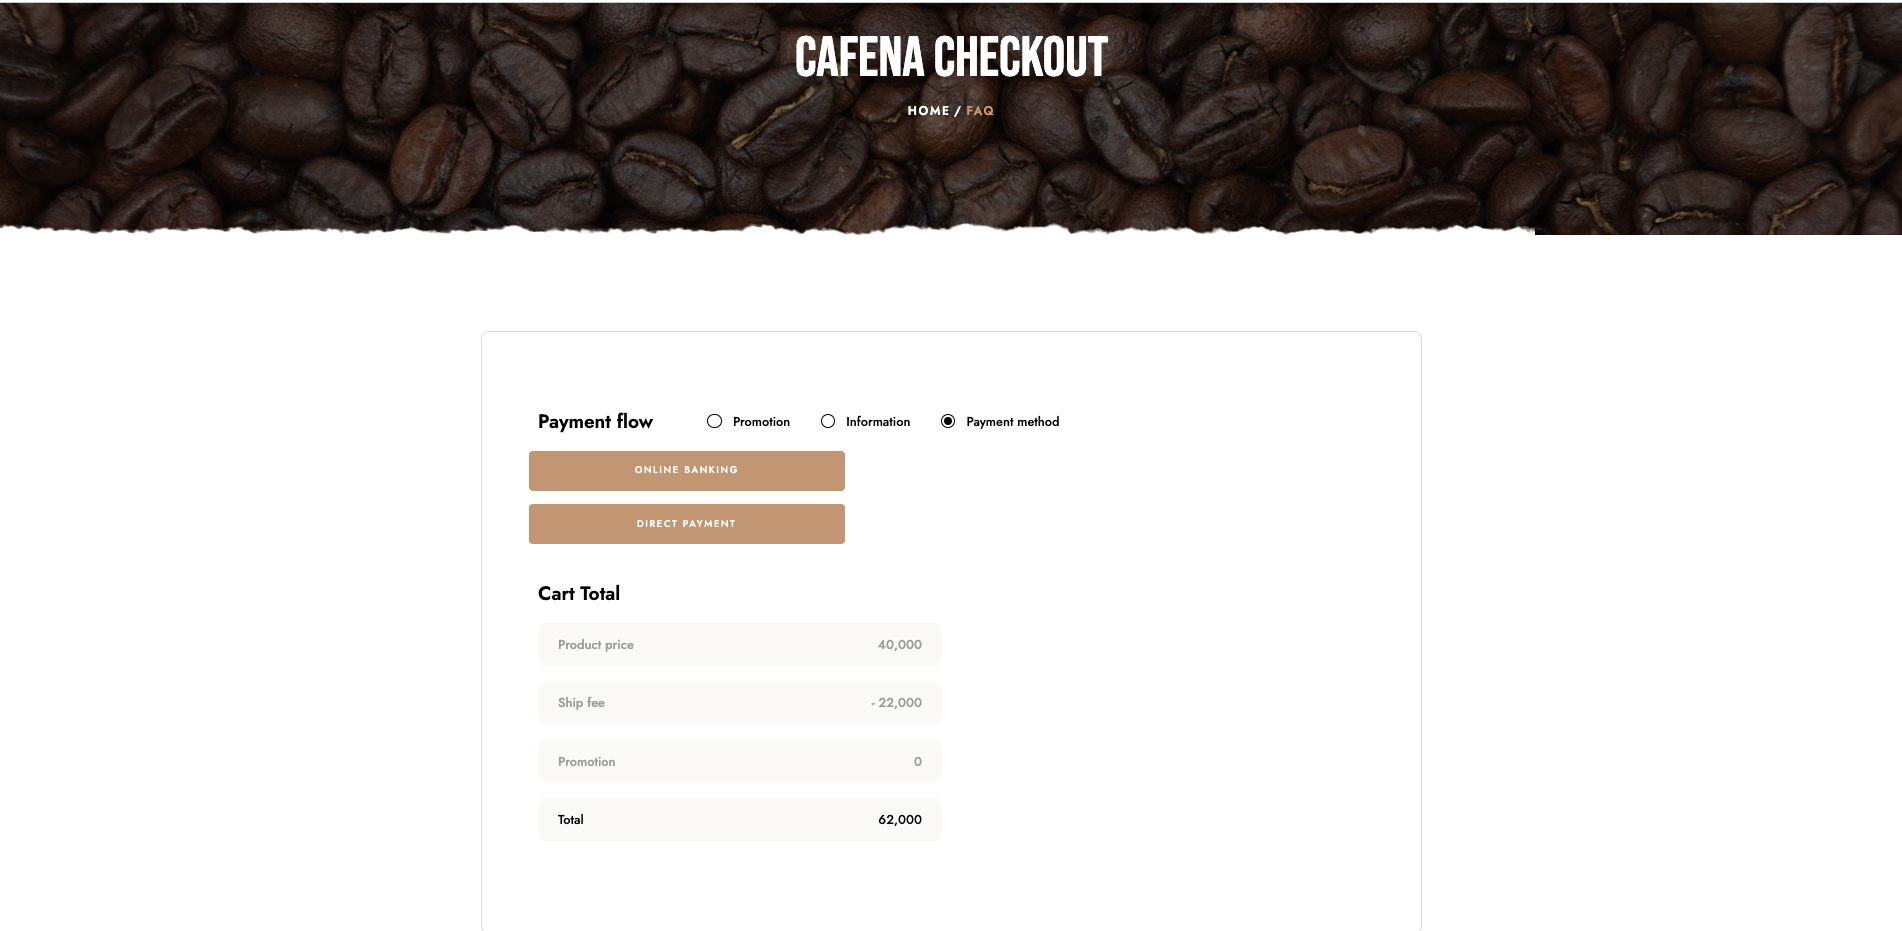
\includegraphics[width=0.7\textwidth]{Demo/Cart2.png}
    \label{fig:cart2page}
\end{figure}
3. The website processes the order, charges the user's payment method, and displays an order confirmation page with the order details. \\
4. The user reviews the order details and can choose to continue shopping or exit the website.
\subsection{View order history}
1. User must login first to see the order history.\\
2. The order history will display.